\section{Analysis}\label{sec:dns_analysis}

With the data we collected, we conducted two major approaches at analysis. The first approach treated every measurement for a recursive server in a give state as equal and gave each state a score based on these measurements aggregated together. The second method first aggregated measurements within one state based on the authoritative state the measurement was made with, which also gave us the opportunity to weight connections to states differently.

\subsection{Distance Normalization}
One of the initial steps in processing the data collected involved adding an additional field for \rtt normalized by the distance between the points being connected. As mentioned earlier in this report, by normalizing for distance, we can form another measurement that allows for analysis of connectivity as related to the \textit{ideal} speed of connection, the speed of light.

Additionally, calculating the speed of the connection, not just the total \rtt, allowed us to filter out measurements that were faster than the speed of light. Such measurements were likely the result of anomalous latency readings, causing the calculated \rtt to be far lower than physically possible. In total, this initial filter eliminated 418,625 measurements (7.5\%) from the total dataset.

\subsection{Data Characterization}

\Cref{fig:dns_analytics_median_dist} shows the distribution of the median true \rtt values for all locations. It shows that the data takes on a bimodal distribution with peaks around 45ms and 68ms with a heavy bias towards the former.

\begin{figure}[htb]
    \centering
    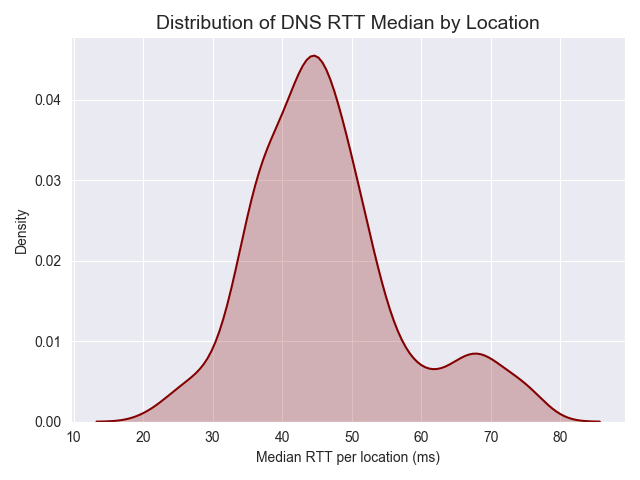
\includegraphics[width=0.75\textwidth]{images/dns/dist_raw_data/dns_rtt_median_distribution.png}
    \caption{DNS RTT median distribution}
    \label{fig:dns_analytics_median_dist}
\end{figure}

\subsubsection{Normalized RTT}

After normalizing by distance, the bimodality all but disappears, as \cref{fig:dns_analytics_norm_median_dist} shows. In this chart, the distribution pears around 30km/ms.

\begin{figure}[htb]
    \centering
    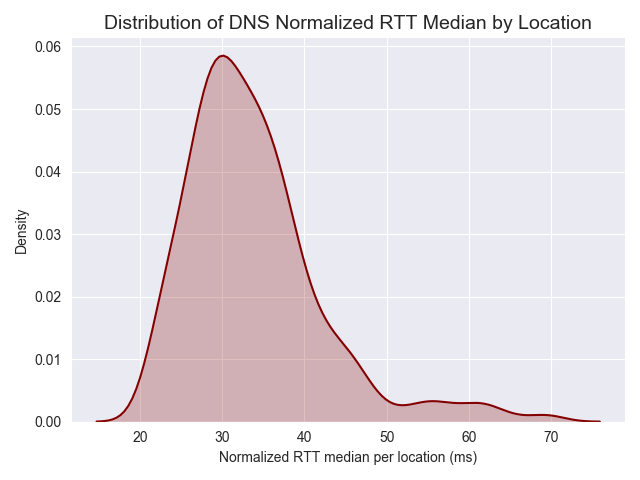
\includegraphics[width=0.75\textwidth]{images/dns/dist_raw_data/dns_norm_rtt_median_distribution.png}
    \caption{DNS normalized RTT median distribution}
    \label{fig:dns_analytics_norm_median_dist}
\end{figure}

\subsection{Heat Maps}

\Cref{fig:dns_true_rtt_heatmap} shows a heatmap based on true \dns \rtt measurements. This map shows that a significant portion of Western US has poor \dns \rtts. In contrast to the West, a majority of the the East Coast performs better. As we discuss later, this is likely due to the higher quantity of authoritative servers present in the East. Another highlight is that the South is rather inconsistent: Mississippi is probably the most homogeneous in being bad, but Alabama, Georgia, Louisiana, Tennessee, Missouri, and even eastern Texas are rather "splotchy", for lack of a better term.

\begin{figure}[htb]
    \centering
    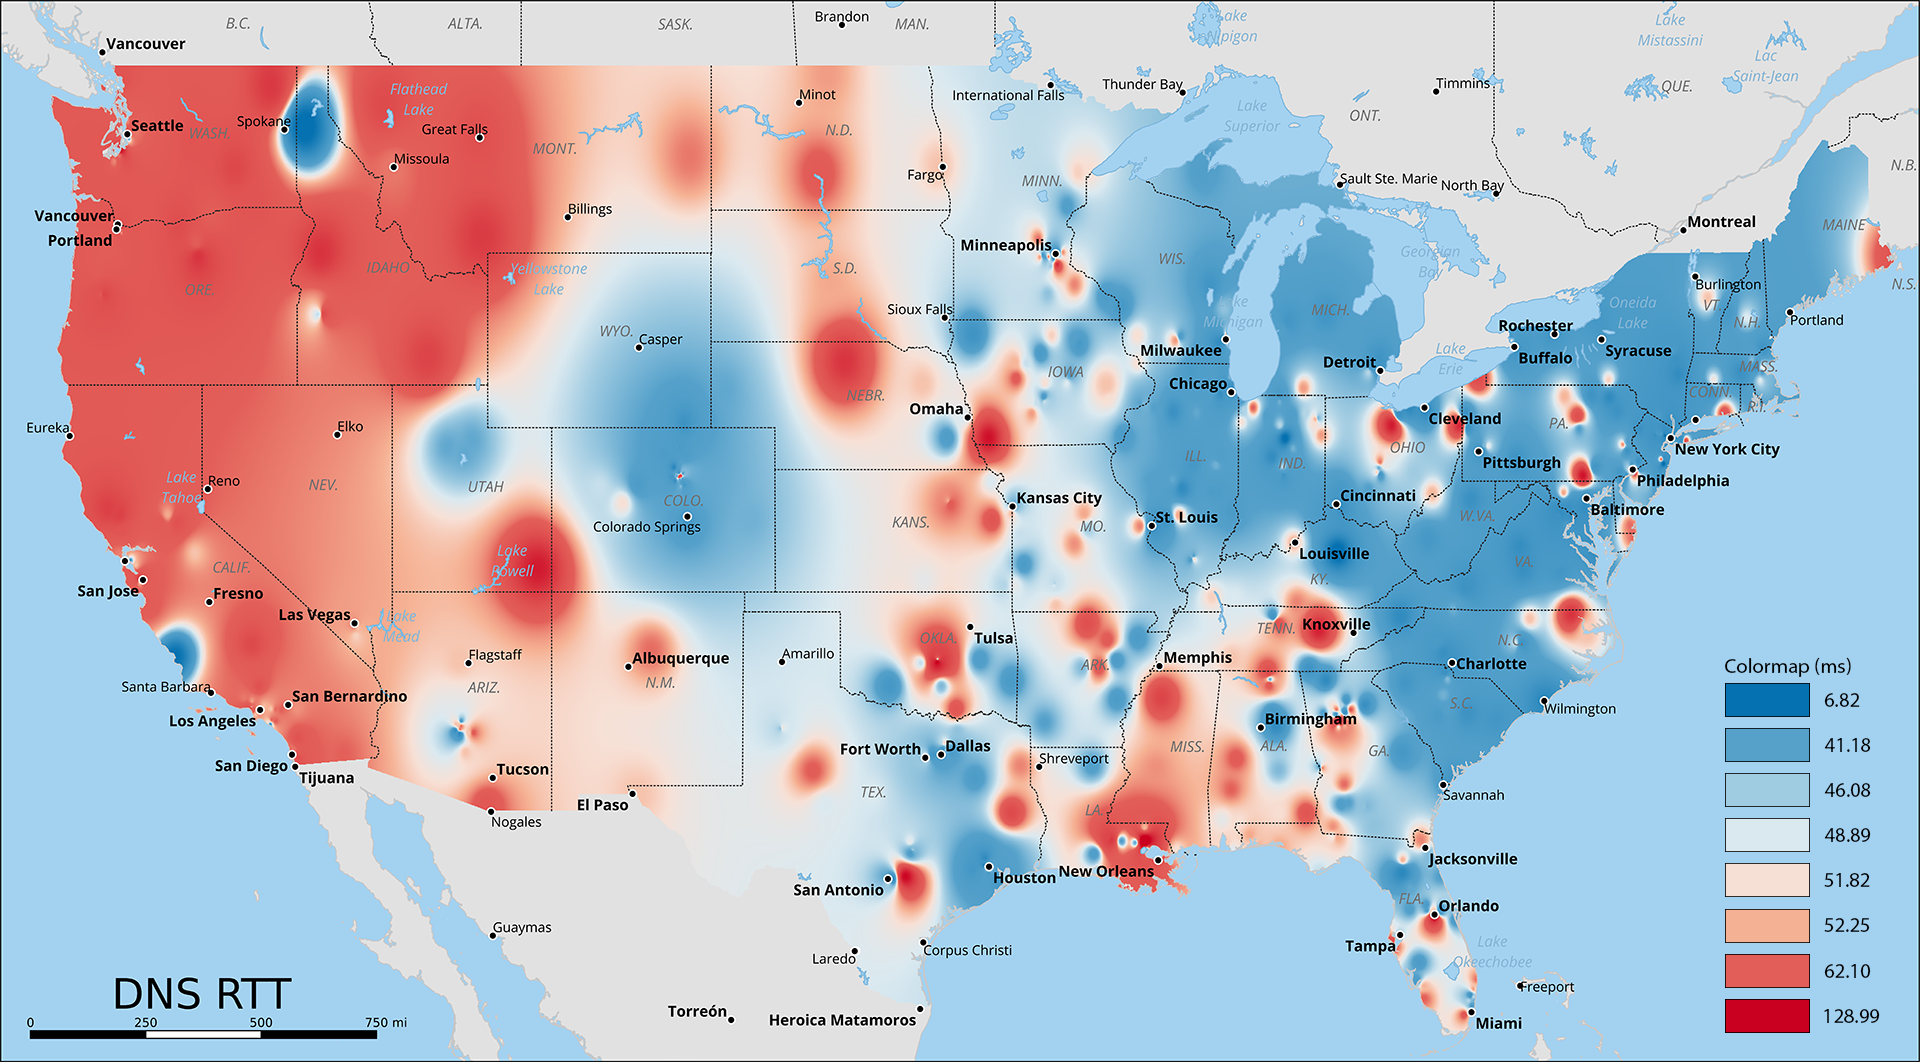
\includegraphics[width=0.75\textwidth]{images/dns/heatmaps/dns_rtt_idw.png}
    \caption{DNS true RTT heatmap}
    \label{fig:dns_true_rtt_heatmap}
\end{figure}

\Cref{fig:dns_normalized_rtt_heatmap} shows a similar heatmap, but for distance normalized \dns \rtt data. In stark contrast to the prior map, the West coast displays significantly better performance - likely due to the distance to eastern authoritative servers being cancelled out. The Midwest and mid-Atlantic regions fare much worse, while the South is far more consistent in its poor results. The two main regions that remain consistent between the two maps are the North East and Colorado/Wyoming.

\begin{figure}[htb]
    \centering
    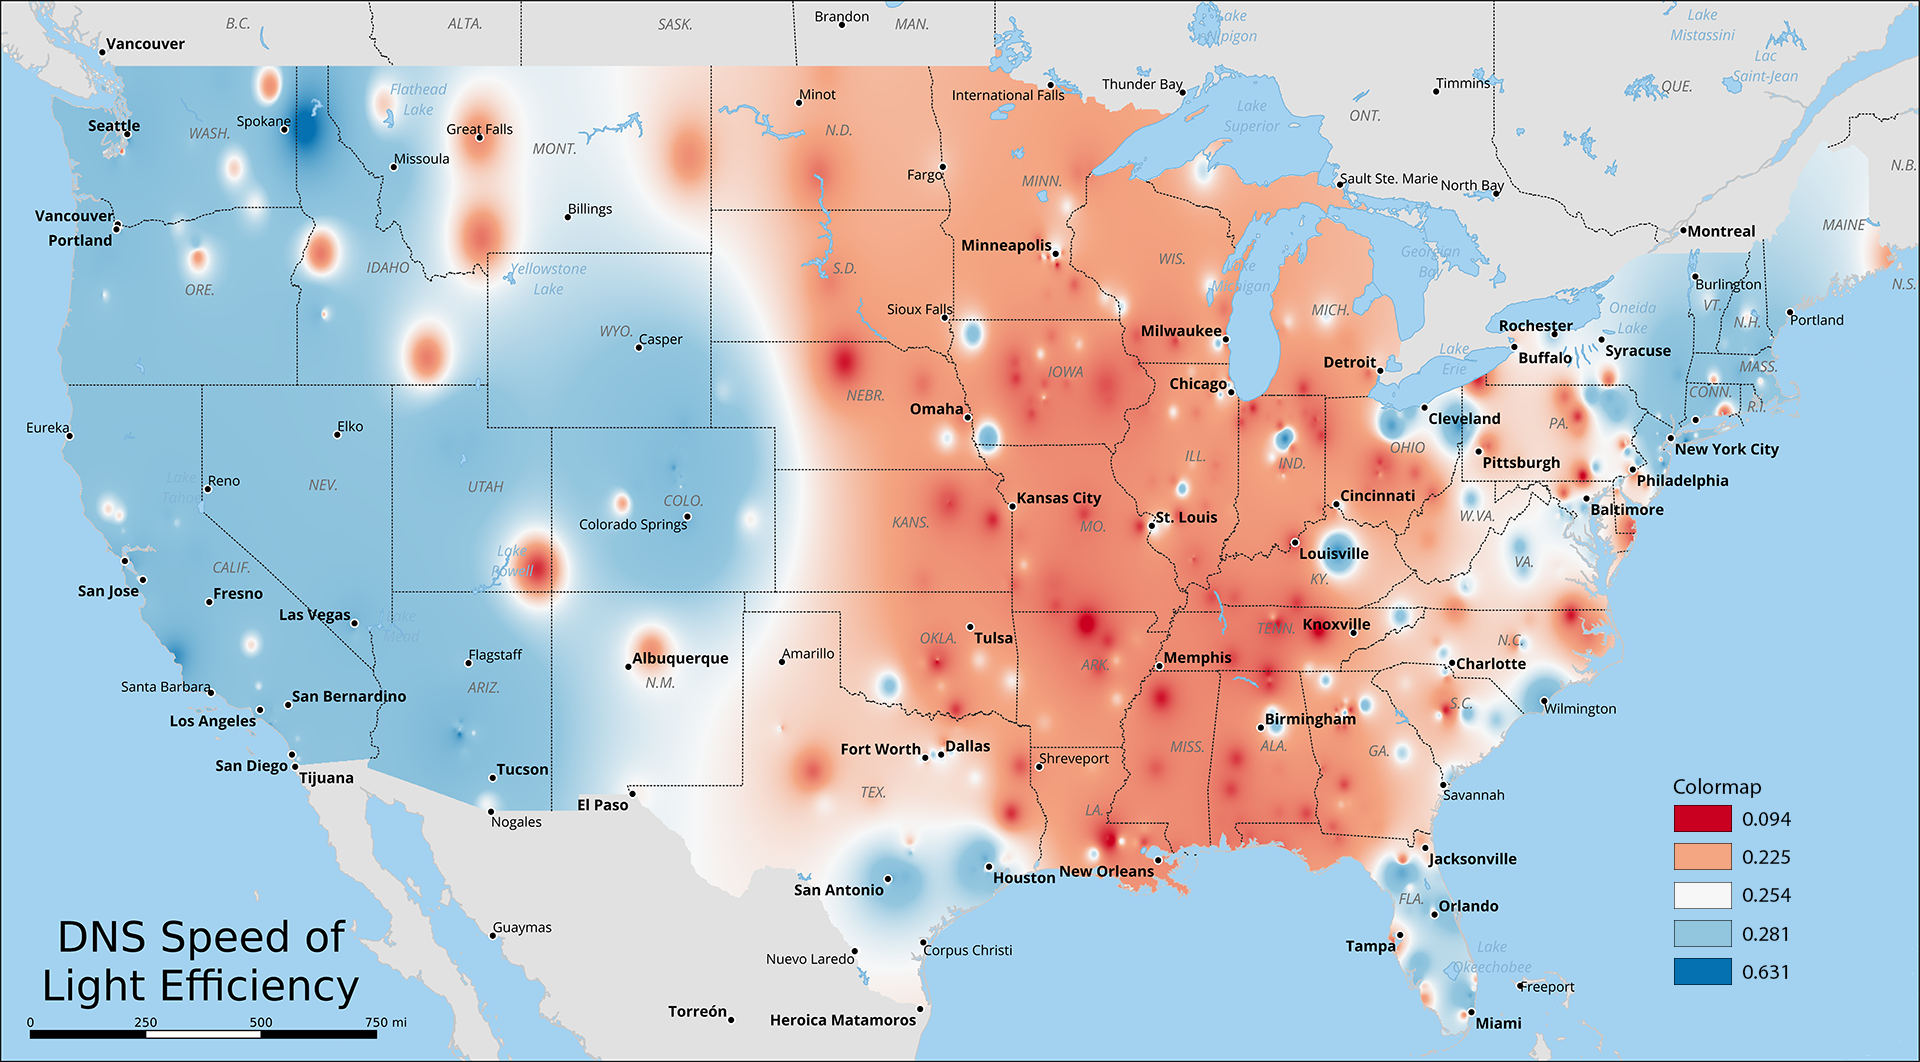
\includegraphics[width=0.75\textwidth]{images/dns/heatmaps/dns_speed_of_light_idw.png}
    \caption{DNS normalized RTT heatmap}
    \label{fig:dns_normalized_rtt_heatmap}
\end{figure}

\subsection{Aggregation by Server Pairs}
Since there we multiple data points for each recursive-authoritative server pair, the first step in aggregating the data was to aggregate by these server pairs. To do this, we removed points within each pair that had a z-score greater than a given threshold \texttt{z} as these were considered outliers within their pairs. We then computed the \cv of each pair with the remaining values and discarded any pairs with a result greater than a given threshold \texttt{v} - these pairs did not have consistent measurements and were considered unreliable.

\begin{table}[htb]
    \centering
    \begin{tabular}{ l|l|l  }
      & \textbf{True \rtt records dropped} & \textbf{Normalized \rtt records dropped} \\
     \hline
      \texttt{z=3} & 92,553/5,188,421 (1.8\%) & 63,008/5,188,421 (1.2\%) \\
      \texttt{z=2} & 269,651/5,188,421 (5.2\%) & 237,353‬/5,188,421 (4.6\%) \\
      \texttt{z=1} & 1,362,184/5,188,421 (26.3\%) & 1,389,031‬/5,188,421 (26.8\%) \\
     \hline
    \end{tabular}
    \caption{DNS Z-score filtering}
    \label{tab:dns_z_filtering}
\end{table}

\begin{table}[htb]
    \centering
    \begin{tabular}{p{1.6cm}|p{4cm}|p{4cm}|p{4cm}}
         & \texttt{z=3} (\texttt{n=381,333}) & \texttt{z=2} (\texttt{n=381,333}) & \texttt{z=1} (\texttt{n=381,333}) \\
        \hline
        \texttt{v=0.05} & 193,099 (50.6\%)  & 167,618 (44.0\%) & ‭92,799 (24.3\%) \\
        \texttt{v=0.10} & 111,294 (29.2\%) & 92,023 (24.1\%) & 40,889 (10.7\%)‬\\
        \texttt{v=0.20} & 52,239 (13.7\%) &  40,353 (10.6\%) & 13,262 (3.5\%)\\
        \texttt{v=0.50} & 9,330 (2.4\%) &  6,333 (1.7\%) & 1,809 (0.5\%)\\
        \texttt{v=1.00} & 1,741 (0.5\%) &    766 (0.2\%) & 176 (\textapprox0.0\%) \\
        \hline
    \end{tabular}
    \caption{True RTT DNS pair CV filtering}
    \label{tab:dns_unnorm_cv_filtering}
\end{table}

\begin{table}[htb]
    \centering
    \begin{tabular}{p{1.6cm}|p{4cm}|p{4cm}|p{4cm}}
         & \texttt{z=3} (\texttt{n=382,963}) & \texttt{z=2} (\texttt{n=382,963}) & \texttt{z=1} (\texttt{n=382,963}) \\
        \hline
        \texttt{v=0.05} & 192,522 (50.3\%) & 166,514 (43.5\%) & 87,383 (22.8\%) \\
        \texttt{v=0.10} & 109,493 (28.6\%) & 89,906 (23.5\%) & 35,553 (9.3\%) \\
        \texttt{v=0.20} & 48,414 (12.6\%) & 37,623 (9.8\%) & 10,579 (2.8\%) \\
        \texttt{v=0.50} & 6,304 (1.6\%) & 4,570 (1.2\%) & 1,314 (0.3\%) \\
        \texttt{v=1.00} & 1,038 (0.3\%) &    415 (0.1\%) & 126 (\textapprox0.0\%) \\  
    \end{tabular}
    \caption{Normalized RTT DNS pair CV filtering}
    \label{tab:dns_norm_cv_filtering}
\end{table}

We chose to proceed with \texttt{v=1.0} and \texttt{z=2}, which left the vast majority of pairs in the data set excluding only the most inconsistent measurements. The reasoning behind this is that we are not just interested in stable connections - so we left potentially unstable or inconsistent measurements in the data set.

\subsection{Aggregating Pairs by Recursive Server State}

One option to further aggregate the pair data is to group it by the location of the recursive server in each pair. This results in a list of \rtts, either true or normalized by distance, that can be aggregated into a single value for each state. This is one way of making comparisons between states.

\subsubsection{Initial State Rankings}

\Cref{tab:dns_only_recursive_initial_state_rankings} shows the results of ranking states by the median of each measurement in that state. There are two different rankings, one each for the true \rtt and the distance normalized \rtt, based on data filtered with \texttt{z=2} and \texttt{v=1.0}. As with all \dns data, there is no ranking for Rhode Island.

\begin{longtable}{lrr||lrr}
% \toprule
  \multicolumn{3}{c||}{\textbf{True RTT}} & \multicolumn{3}{c}{\textbf{Normalized RTT}} \\
     \textbf{State} &  \textbf{Rank} & \textbf{(ms)} & \textbf{State} & \textbf{Rank} & \textbf{(km/ms)} \\
\midrule
\endhead
\midrule
\multicolumn{6}{r}{{Continued on next page}} \\
\midrule
\endfoot
% \bottomrule
\endlastfoot
        WY &    1 &  30.0 &             HI &    1 &  91.0 \\
        VA &    2 &  31.0 &             WY &    2 &  54.5 \\
        DC &    2 &  31.0 &             AK &    3 &  47.4 \\
        WV &    4 &  32.0 &             CA &    4 &  45.5 \\
        NY &    4 &  32.0 &             OR &    5 &  43.9 \\
        NJ &    6 &  33.0 &             NV &    6 &  43.7 \\
        MD &    7 &  34.0 &             CO &    7 &  43.6 \\
        SC &    8 &  34.5 &             NY &    8 &  43.0 \\
        CO &    9 &  38.0 &             UT &    9 &  42.7 \\
        NH &   10 &  38.5 &             ID &   10 &  42.0 \\
        IL &   11 &  39.0 &             WA &   11 &  41.8 \\
        MI &   12 &  40.0 &             NH &   12 &  41.7 \\
        PA &   12 &  40.0 &             AZ &   13 &  41.0 \\
        WI &   12 &  40.0 &             NJ &   14 &  40.9 \\
        NC &   15 &  41.0 &             MA &   15 &  40.7 \\
        TX &   16 &  42.0 &             VA &   16 &  37.1 \\
        MA &   16 &  42.0 &             FL &   17 &  37.0 \\
        OH &   16 &  42.0 &             TX &   18 &  36.8 \\
        IN &   19 &  43.0 &             MD &   19 &  36.4 \\
        GA &   19 &  43.0 &             DC &   20 &  35.8 \\
        MN &   21 &  45.0 &             SC &   21 &  34.6 \\
        OK &   22 &  46.0 &             CT &   22 &  33.6 \\
        MO &   22 &  46.0 &             PA &   23 &  33.3 \\
        LA &   22 &  46.0 &             NC &   24 &  32.4 \\
        AR &   22 &  46.0 &             MT &   25 &  32.0 \\
        CT &   22 &  46.0 &             VT &   26 &  31.6 \\
        FL &   27 &  47.0 &             MI &   27 &  31.5 \\
        IA &   28 &  48.0 &             WI &   28 &  30.6 \\
        KY &   29 &  49.0 &             WV &   29 &  30.6 \\
        NE &   30 &  49.5 &             NM &   30 &  30.4 \\
        UT &   31 &  50.0 &             MN &   31 &  30.0 \\
        VT &   32 &  51.0 &             ME &   32 &  29.8 \\
        TN &   33 &  52.0 &             GA &   33 &  29.6 \\
        AL &   34 &  53.0 &             ND &   34 &  29.4 \\
        AZ &   34 &  53.0 &             LA &   35 &  29.3 \\
        DE &   34 &  53.0 &             OK &   36 &  28.9 \\
        NV &   34 &  53.0 &             SD &   37 &  28.6 \\
        ID &   38 &  54.0 &             NE &   38 &  28.3 \\
        SD &   39 &  56.0 &             IL &   39 &  28.1 \\
        KS &   39 &  56.0 &             DE &   40 &  27.6 \\
        ND &   41 &  59.0 &             MO &   41 &  26.4 \\
        CA &   42 &  59.5 &             AR &   42 &  26.2 \\
        NM &   43 &  60.0 &             OH &   43 &  25.4 \\
        HI &   43 &  60.0 &             IA &   44 &  25.0 \\
        MS &   45 &  62.0 &             AL &   45 &  24.5 \\
        OR &   46 &  65.0 &             IN &   46 &  24.4 \\
        WA &   47 &  67.0 &             KS &   47 &  22.9 \\
        ME &   48 &  67.5 &             KY &   48 &  21.9 \\
        MT &   49 &  71.0 &             TN &   49 &  21.6 \\
        AK &   50 &  99.2 &             MS &   50 &  20.4 \\
        RI &   -- &    -- &             RI &   -- &    -- \\
        \caption{Initial State Rankings -- Recursive Location Aggregation}
        \label{tab:dns_only_recursive_initial_state_rankings}
\end{longtable}


Notably, \cref{tab:dns_only_recursive_initial_state_rankings} indicates that Wyoming ranks in the top five for both rankings. No other state appears performs so consistently well. Additionally, the rankings show that while Hawaii and Alaska rank near or at the bottom for true \rtt, both states appear near the top of the normalized ranking. This shows that while the some states, Alaska and Hawaii in particular, may be inherently unconnected from the rest of the United States, the quality of their connection could be relatively high and merely dominated by sheer distances.

\subsubsection{Evaluating State Rankings}

To determine the validity of the rankings proposed above we used the Kruskal-Wallis test to determine whether there was evidence that datasets for different states came from different distributions. If we cannot reject the null hypothesis that they are from the same distribution, we cannot rank them in distinct positions. After running Kurskals between the datasets for each of the 49 states and DC, we used a p value threshold of 0.05 to determine if we could differentiate two states from each other. 

% \begin{figure}[h]
\begin{wrapfigure}[28]{L}{0.65\textwidth}
    \centering
    \includesvg[width=0.65\textwidth]{images/dns/analysis_no_auth_agg/rtt/no_auth_agg_true_rtt_graph.svg}
    \caption{DNS true RTT indistinguishability graph}
    \label{fig:dns_true_rtt_indistinguishable_states_graph}
\end{wrapfigure}
% \end{figure}

For true \rtt, \cref{fig:dns_true_rtt_indistinguishable_states_graph} shows a graph with a node for each of the 49 states and DC and a link between each pair of nodes where the Kruskal-Wallis test between the two yielded a p value greater than 0.05, indicating that there is no evidence of a difference between the two states. Each the y-position for each state in the graph is dictated by its ranking in the the initial ranking table (ties were broken up arbitrarily for readability and the x-position is arbitrary). 

Note that the top seven states in the true \rtt ranking in \cref{tab:dns_only_recursive_initial_state_rankings}, WY, VA, DC, WV, NY, NJ, and MD, form a distinct sub graph. Similarly, the states ranked \#9-12, IL, CO, NH, and MI, form another distinct sub graph. This indicates that while the states that make up these two groups cannot be distinguished from one another (i.e. there is no evidence that Wyoming is better than Virginia), we can state the the entirety of the first group is better than the entirety of the second group.

Similar to the groups at the top of the ranking, there are distinct groups at the bottom. Kruskals identified Alaska, \#50, as entirely different. However, the six preceding states ranked \#43(t) to \#49, HI, MS, OR, WA, ME, and MT, are a distinct sub graph, as are the three states preceding them, ND, NM, and HI. Note that in the initial ranking, New Mexico and Hawaii are tied for \#43, but are identified as distinct using Kruskals.

Also notable is Louisiana: the state ranks \#22(t), but is labeled as indistinguishable from Arizona, \#34(t), and Nevada, \#34(t).

\begin{figure}[htb]
    \centering
    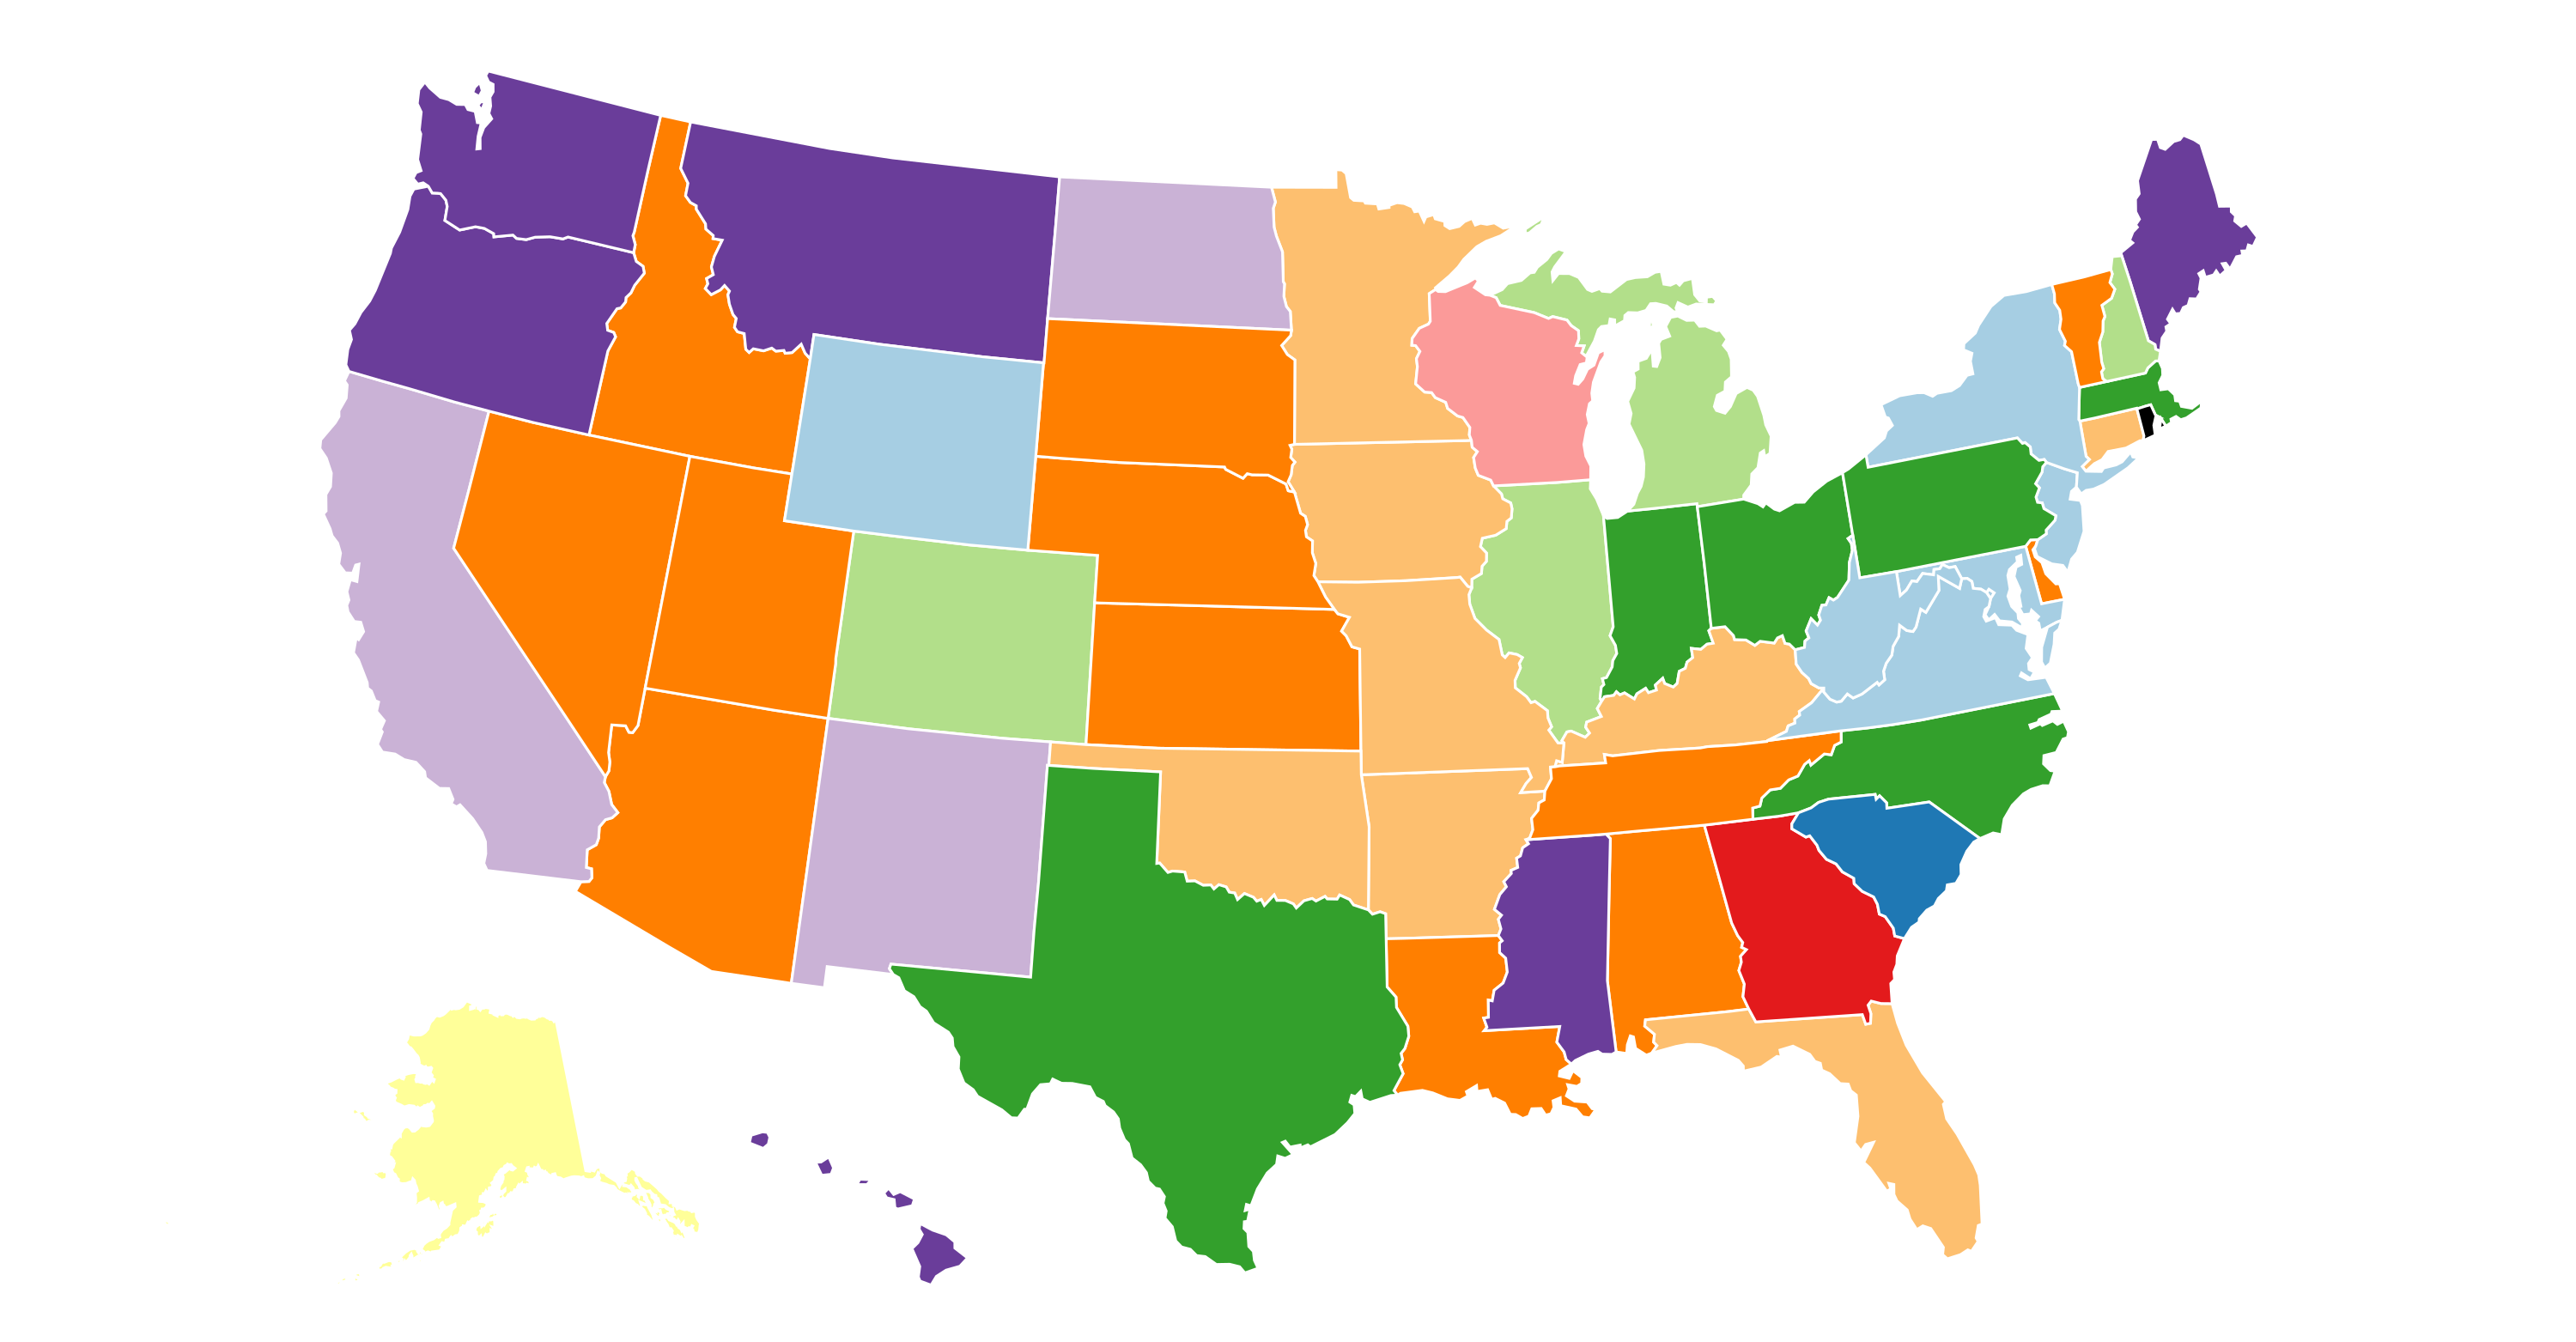
\includegraphics[width=0.75\textwidth]{images/dns/analysis_no_auth_agg/rtt/no_auth_distinct_rtt_map.png}
    \caption{DNS true RTT state groupings}
    \label{fig:dns_true_rtt_indistinguishable_states_map}
\end{figure}

\Cref{fig:dns_true_rtt_indistinguishable_states_map} maps the each distinct sub graph to a separate color (graphs are numbered by in the order of their highest ranked consituent state). This highlights some patterns and some oddities. For example, seven of the top eight states, represented by groups 1 and 2, are located on the East Coast, with Wyoming being the odd state out. The Midwest and the western Mountain region are dominated by states in groups 7 and 8. The Great Lakes region consists primarily of states in groups 3 and four. The West Coast and Hawaii did not fair as well as the East Coast with California, Oregon, and Washington (and Hawaii) in groups 9 and 10. Meanwhile, the South is a bit of a "hodge-podge" of groups, indicating a lack of consistency there.

\begin{figure}[htb]
    \centering
    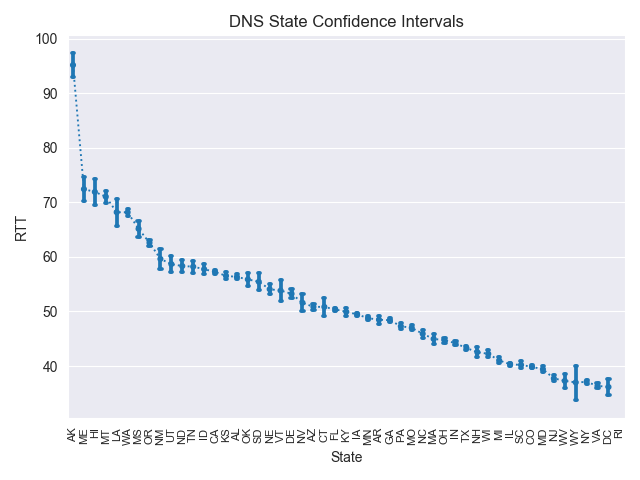
\includegraphics[width=0.75\textwidth]{images/dns/analysis_no_auth_agg/rtt/no_auth_agg_rtt_confidence.png}
    \caption{DNS true RTT confidence intervals}
    \label{fig:dns_true_rtt_confidence_intervals}
\end{figure}

Finally, for true \rtt, \cref{fig:dns_true_rtt_confidence_intervals} shows bootstrapped confidence intervals for each state. With a few exceptions, bounds are fairly tight, indicating high confidence that the ranking listed in \cref{tab:dns_only_recursive_initial_state_rankings} is reliable. One of the notable exceptions is Wyoming, which has a much higher confidence interval than its neighbors in the "good" \rtt region. One possible cause for this may be the fact that Wyoming only had one recursive server in it. However, this was also the case for other servers that did not exhibit the behavior that Wyoming did.

Similar to the graph for true \rtt, \cref{fig:dns_normalized_rtt_indistinguishable_states_graph} is a graph of states in the normalized \rtt ranking that are indistinguishable. This graph includes a much larger and messier middle group consisting of 27 states. Hawaii, ranked \#1 is an independent node, as is California at \#4, with Alaska and Wyoming forming a pair between these two. At the bottom, Mississippi is distinctly alone. The second largest distinct subgroup consists of 10 states spanning from \#5 to \#15, with Utah distinct from all of them, but ranked \#9.

% \begin{figure}[htb]
\begin{wrapfigure}[27]{R}{0.50\textwidth}
    \centering
    \includesvg[width=0.50\textwidth]{images/dns/analysis_no_auth_agg/rtt_normalized/no_auth_agg_norm_rtt_graph.svg}
    \caption{DNS normalized RTT indistinguishable states graph}
    \label{fig:dns_normalized_rtt_indistinguishable_states_graph}
\end{wrapfigure}
% \end{figure}

Overall, \cref{fig:dns_normalized_rtt_indistinguishable_states_graph} shows that while there are more completely distinct states in the normalized rankings, the states in the middle of the pack are dominated by a single large cluster.

Mapping the distinct sub graphs for normalized \dns \rtt shows a majority of the large, mid ranking sub graph is on the East Coast and in the Midwest, with some states in the Mountain region. The West Coast is comprised entirely of states in groups 3 and 4, which also contain some states in the North East.

\begin{figure}[htb]
    \centering
    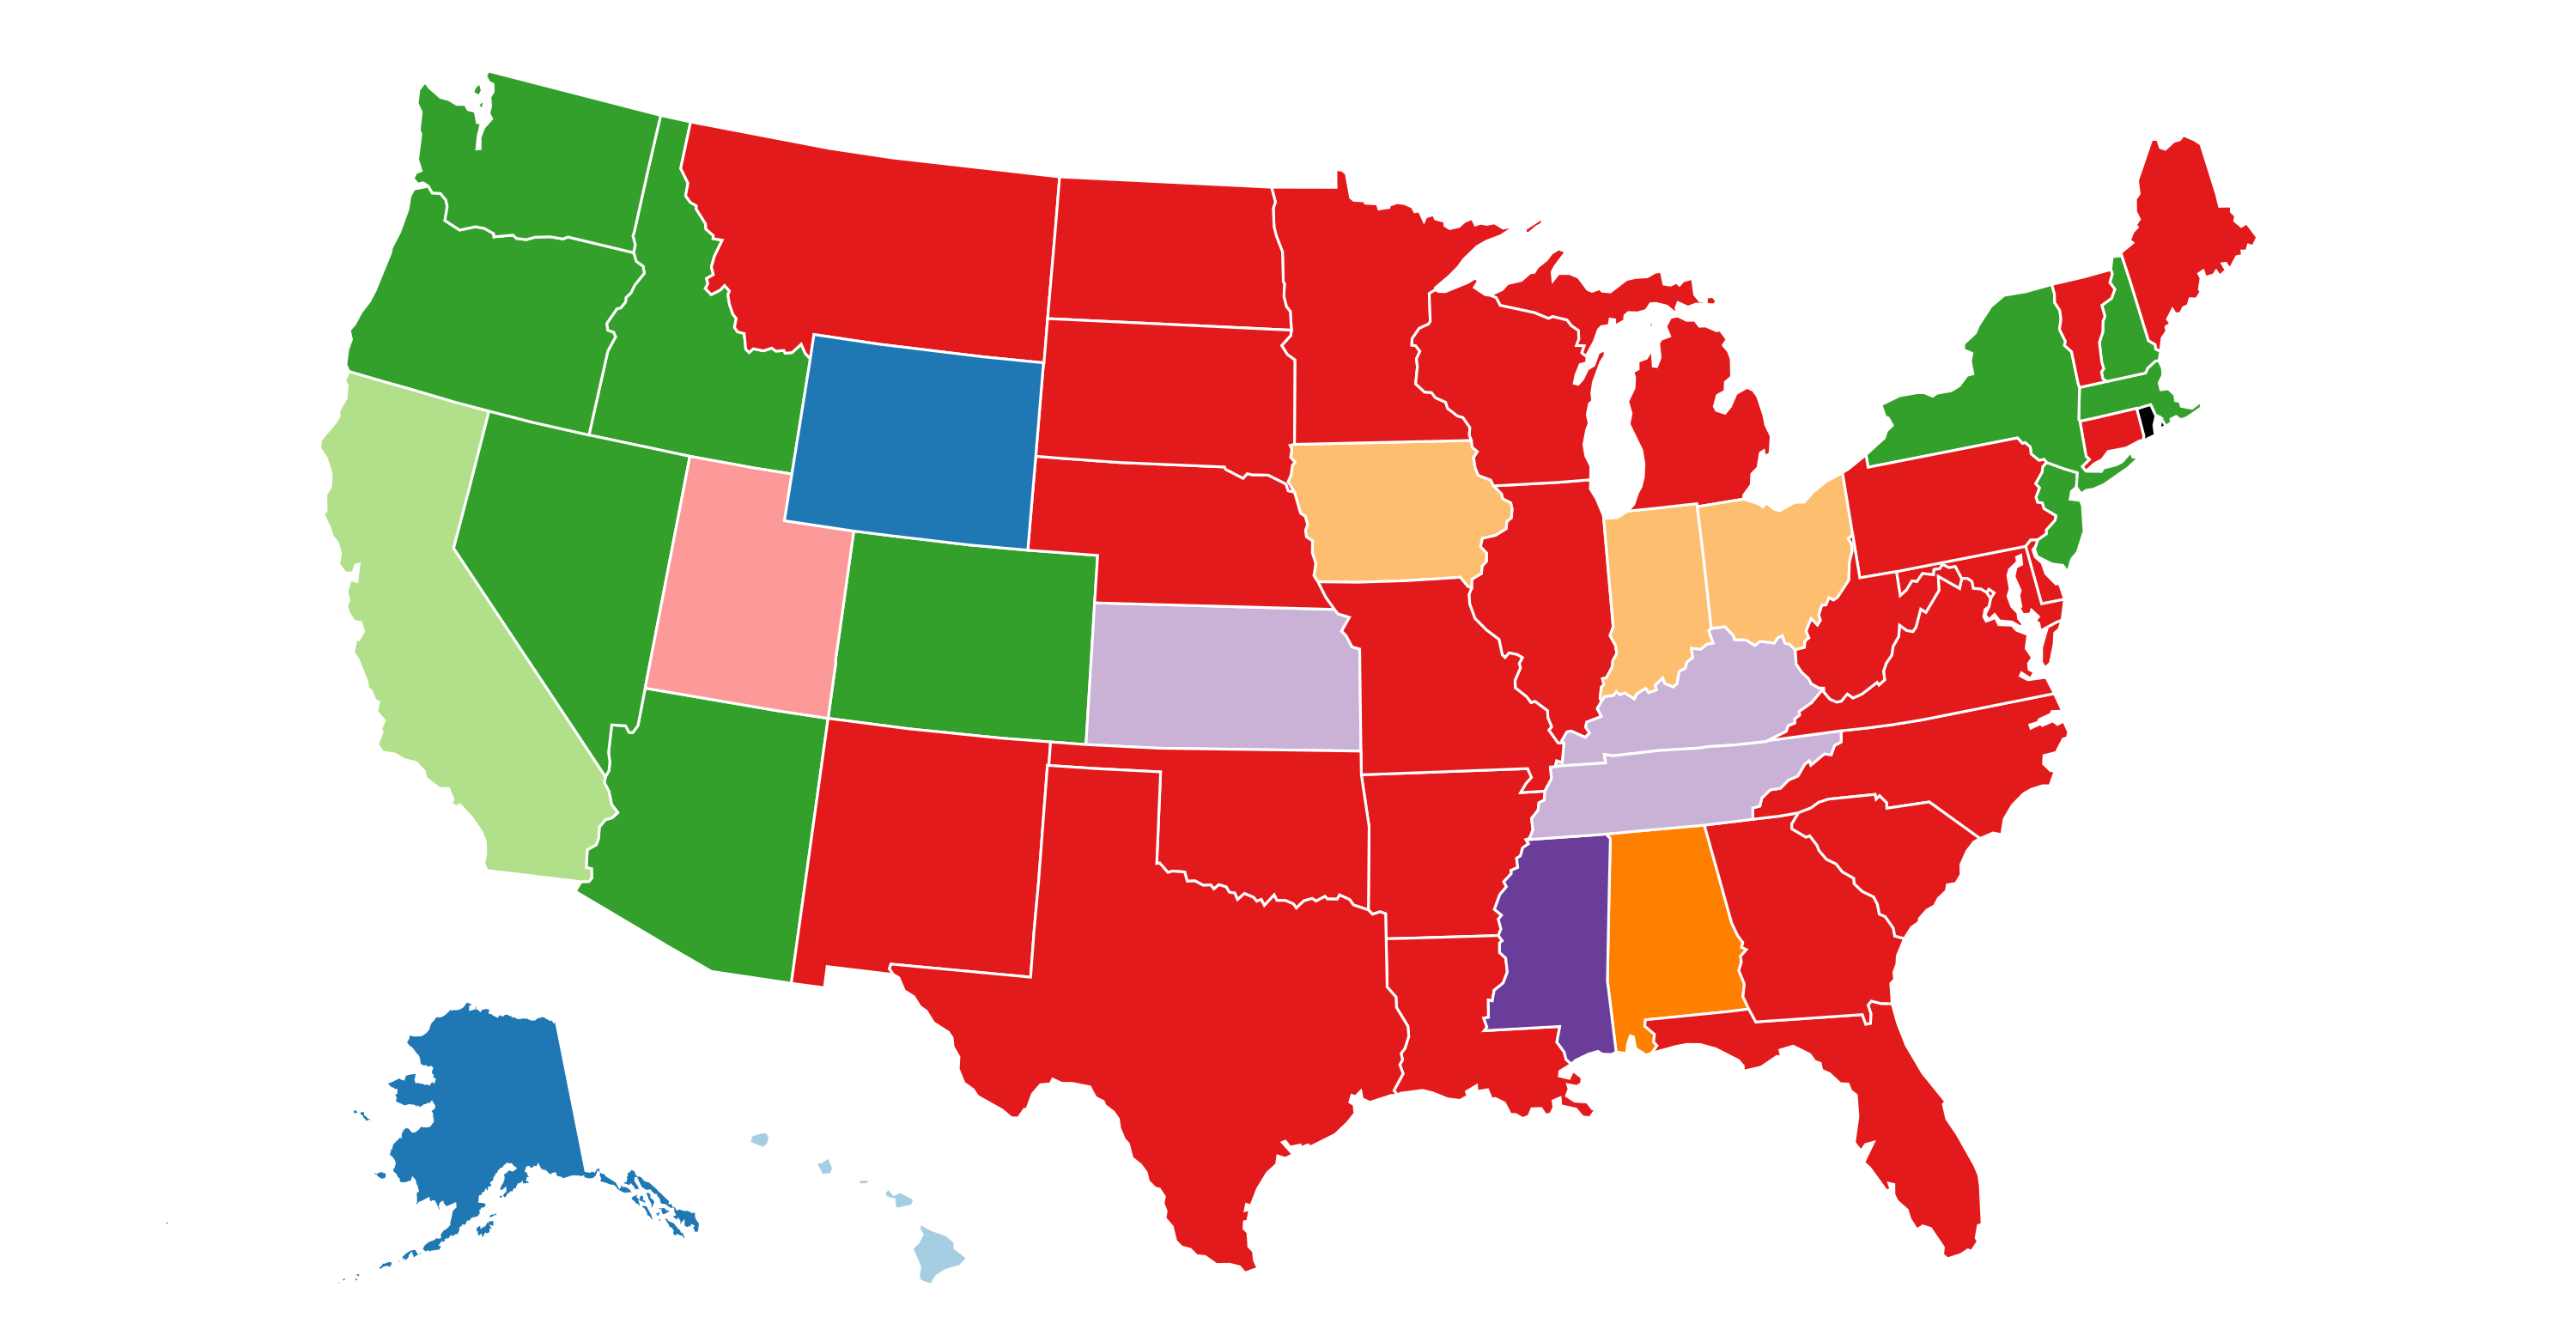
\includegraphics[width=0.75\textwidth]{images/dns/analysis_no_auth_agg/rtt_normalized/no_auth_distinct_norm_rtt_map.png}
    \caption{Normalized RTT indistinguishability graph}
    \label{fig:dns_normalized_rtt_indistinguishable_states_map}
\end{figure}

\subsection{Aggregation by Authoritative State then Recursive State}

One shortcoming of aggregating pairs directly by the location of the recursive server is that this inherently weights the data by the number of authoritative servers in a single state. To compensate, this analysis approach first groups and aggregates by recursive server and authoritative server location. 

Given the presence of authoritative servers in every state, this creates a list of 51 measurements for each state with a recursive server. For example, all measurements between a recursive server in California and an authoritative server in Massachusetts are aggregated into a single measurement (using median) for California. This is then done for every other state with measurements from California, giving California a 51 measurement dataset, and then repeated for each state with a recursive server. 

To get a final value for a given state, each of these 51 measurements is averaged. Back to the example of California, this gives each state with measurements from California an equal weight in the final value for California. 

However, prior to averaging the 51 measurements for each state, we had the option of applying weights to the values. Again with the California example, we could apply a weight to the aggregated measurement between it and Massachusetts based on Massachusetts' population, \gdp, or other metric. For example, Massachusetts has a high population than Wyoming, so with a population based weighting scheme, the measurement to Massachusetts is valued higher than the measurement to Wyoming.

We chose to proceed with unweighted and population weighted aggregations. Weighting by population gives higher value to connections with states that have greater populations. Essentially, this creates a proxy for how well connected people in one state are to all other people in the United States.

\subsubsection{State Rankings}

\Cref{tab:dns_auth_initial_state_rankings} shows rankings based on this aggregation method, unweighted and population weighted, for both true \dns \rtt and normalized \dns \rtt. There are some shared patterns with the previous aggregation rankings: Wyoming ranks highly in all four, Alaska and Hawaii are at the bottom in both true \rtt metrics but rise to top when looking at the normalized rankings. Under true \rtt, all weighted \rtt values are lower than the values at the same rank in the unweighted column. This indicates states with higher populations have generally lower values than their counterparts, driving down the weighted metrics.

\todo{Units}
\begin{longtable}{lrr|lrr||lrr|lrr}
\toprule
  \multicolumn{6}{c||}{True RTT} & \multicolumn{6}{c}{Normalized RTT} \\
\multicolumn{3}{c|}{Unweighted} & \multicolumn{3}{c||}{Pop. Weighted} & \multicolumn{3}{c|}{Unweighted} & \multicolumn{3}{c}{Pop. Weighted} \\
     State & Rank & Value &         State & Rank &  Value &          State & Rank &  Value &         State & Rank &  Value \\
\midrule
\endhead
\midrule
\multicolumn{12}{r}{{Continued on next page}} \\
\midrule
\endfoot
\bottomrule
\endlastfoot
        VA &    1 &  39.6 &            WI &    1 &   49.4 &             HI &    1 &  106.9 &            WY &    1 &  147.6 \\
        NY &    2 &  40.3 &            CO &    2 &   49.9 &             WY &    2 &   71.7 &            HI &    2 &  125.4 \\
        WY &    3 &  40.9 &            IL &    3 &   50.0 &             VT &    3 &   50.8 &            VT &    3 &   72.1 \\
        WV &    3 &  40.9 &            WV &    4 &   50.3 &             AK &    4 &   46.8 &            AZ &    4 &   69.1 \\
        MD &    5 &  41.2 &            UT &    5 &   51.0 &             CA &    5 &   46.7 &            CA &    5 &   63.3 \\
        DC &    6 &  42.0 &            MI &    6 &   51.4 &             NV &    6 &   46.2 &            NV &    6 &   60.7 \\
        NJ &    7 &  42.3 &            TX &    7 &   51.5 &             UT &    7 &   46.1 &            CT &    7 &   59.6 \\
        WI &    8 &  43.5 &            MN &    8 &   51.9 &             AZ &    8 &   43.5 &            OR &    8 &   57.6 \\
        IL &    9 &  43.7 &            SC &    9 &   53.8 &             CT &    9 &   43.4 &            UT &    9 &   56.9 \\
        SC &    9 &  43.7 &            NY &   10 &   54.1 &             OR &   10 &   43.3 &            WA &   10 &   52.5 \\
        MI &   11 &  43.8 &            OH &   11 &   54.3 &             WA &   11 &   41.9 &            NM &   11 &   50.1 \\
        CT &   11 &  43.8 &            IN &   12 &   54.4 &             NY &   12 &   40.3 &            AK &   12 &   49.5 \\
        CO &   13 &  44.7 &            VA &   13 &   54.7 &             CO &   13 &   39.8 &            NY &   13 &   49.0 \\
        UT &   14 &  46.4 &            MO &   14 &   54.9 &             NM &   14 &   38.8 &            CO &   14 &   47.0 \\
        NH &   15 &  47.2 &            NJ &   15 &   55.3 &             NH &   15 &   38.7 &            NH &   15 &   46.9 \\
        TX &   15 &  47.2 &            AR &   16 &   56.0 &             VA &   16 &   37.4 &            VA &   16 &   45.8 \\
        PA &   17 &  47.6 &            CT &   17 &   56.1 &             NJ &   17 &   37.3 &            MT &   17 &   45.7 \\
        NC &   18 &  47.7 &            NM &   18 &   56.4 &             TX &   17 &   37.3 &            DC &   18 &   45.6 \\
        MN &   19 &  48.0 &            WY &   19 &   56.9 &             MD &   19 &   37.1 &            NJ &   18 &   45.6 \\
        OH &   20 &  48.8 &            MD &   20 &   57.1 &             FL &   20 &   36.6 &            MD &   20 &   45.1 \\
        AR &   21 &  49.0 &            PA &   20 &   57.1 &             DC &   20 &   36.6 &            SC &   21 &   42.2 \\
        IN &   22 &  49.1 &            LA &   22 &   57.2 &             SC &   22 &   35.8 &            WV &   22 &   41.7 \\
        GA &   23 &  50.1 &            OK &   23 &   57.5 &             MA &   23 &   33.8 &            NE &   23 &   41.2 \\
        LA &   24 &  50.3 &            GA &   23 &   57.5 &             WV &   24 &   33.4 &            MA &   24 &   40.7 \\
        NM &   25 &  50.7 &            IA &   25 &   57.7 &             MT &   25 &   32.8 &            TX &   25 &   40.2 \\
        MO &   26 &  50.9 &            NV &   26 &   57.8 &             LA &   25 &   32.8 &            FL &   26 &   39.7 \\
        MA &   27 &  51.5 &            DC &   27 &   58.4 &             NE &   27 &   32.5 &            MN &   27 &   38.6 \\
        NE &   28 &  51.8 &            NC &   28 &   58.5 &             NC &   28 &   31.7 &            ID &   28 &   38.5 \\
        NV &   29 &  53.0 &            AZ &   29 &   58.7 &             MI &   29 &   31.3 &            PA &   29 &   37.6 \\
        IA &   30 &  53.2 &            NE &   30 &   60.5 &             ID &   30 &   31.1 &            LA &   30 &   37.2 \\
        OK &   30 &  53.2 &            NH &   31 &   61.1 &             GA &   31 &   31.0 &            NC &   31 &   37.1 \\
        FL &   32 &  54.6 &            KY &   32 &   61.3 &             MN &   32 &   30.9 &            GA &   32 &   36.1 \\
        AZ &   33 &  55.2 &            FL &   33 &   62.8 &             WI &   33 &   30.5 &            MI &   33 &   34.5 \\
        KY &   34 &  55.8 &            MA &   33 &   62.8 &             PA &   34 &   30.4 &            WI &   34 &   34.2 \\
        SD &   35 &  58.6 &            SD &   35 &   63.7 &             AR &   35 &   29.2 &            OH &   35 &   34.0 \\
        TN &   36 &  59.1 &            CA &   36 &   64.1 &             IL &   35 &   29.2 &            AR &   36 &   33.9 \\
        AL &   37 &  59.7 &            ND &   37 &   64.3 &             ND &   37 &   28.4 &            IL &   37 &   33.8 \\
        CA &   38 &  60.0 &            AL &   38 &   65.3 &             OK &   38 &   28.1 &            DE &   38 &   33.1 \\
        ND &   39 &  60.9 &            KS &   39 &   65.9 &             ME &   39 &   27.6 &            OK &   39 &   32.3 \\
        KS &   40 &  62.9 &            TN &   39 &   65.9 &             SD &   40 &   27.2 &            ND &   40 &   32.1 \\
        DE &   41 &  63.5 &            DE &   41 &   68.7 &             MO &   41 &   26.4 &            ME &   41 &   31.9 \\
        OR &   42 &  65.1 &            MT &   42 &   71.5 &             AL &   41 &   26.4 &            SD &   42 &   31.1 \\
        WA &   43 &  66.4 &            WA &   43 &   72.3 &             OH &   43 &   26.3 &            MO &   43 &   30.7 \\
        MT &   44 &  67.4 &            MS &   44 &   72.9 &             IN &   44 &   25.4 &            IN &   43 &   30.7 \\
        MS &   45 &  68.8 &            OR &   45 &   74.3 &             IA &   45 &   24.7 &            AL &   45 &   30.5 \\
        HI &   46 &  70.5 &            HI &   46 &   81.6 &             DE &   46 &   24.6 &            IA &   46 &   28.6 \\
        ID &   47 &  74.9 &            ID &   47 &   82.6 &             KY &   47 &   23.0 &            TN &   47 &   28.1 \\
        ME &   48 &  77.8 &            ME &   48 &   85.1 &             TN &   48 &   22.6 &            KY &   48 &   28.0 \\
        VT &   49 &  83.9 &            AK &   49 &  102.9 &             MS &   49 &   22.2 &            MS &   49 &   26.5 \\
        AK &   50 &  99.1 &            VT &   50 &  104.1 &             KS &   50 &   22.1 &            KS &   50 &   25.8 \\
        RI &   -- &    -- &            RI &   -- &     -- &             RI &   -- &     -- &            RI &   -- &     -- \\
        
%         \caption{Initial State Rankings -- Authoritative Location Aggregation}
%         \label{tab:dns_auth_initial_state_rankings}
\end{longtable}

\subsubsection{Evaluating State Rankings}

As with the previous aggregation method, we began evaluating this approach by using the Kruskal-Wallis test. States were compared against each other using the 51 measurement dataset created by aggregating by the location of authoritative servers.

\Cref{fig:dns_auth_agg_s2s_true_rtt_graphs} shows the results of this analysis for true \rtt, with the unweighted results on the left and the population weighted results on the right. \Cref{fig:dns_auth_agg_s2s_norm_rtt_graphs} does the same for the normalized data. All four show roughly the same thing: with this analysis method, there are very few completely distinct states (Hawaii in the normalized data and Alaska in the unweighted true \rtt data). Overall, the unweighted data for both true \rtt and normalized \rtt show lower inter-connectivity, indicating that states are more distinguishable from each other when the data is not weighted.

\begin{figure}[htb]
    \centering
    \includesvg[width=0.45\textwidth]{images/dns/analysis_auth_agg/rtt/unweighted/analysis_auth_agg_graph_rtt_un.svg}
    \includesvg[width=0.45\textwidth]{images/dns/analysis_auth_agg/rtt/population/analysis_auth_agg_graph_rtt_pop.svg}
    \caption{Unweighted and population weighted rank graphs (true RTT)}
    \label{fig:dns_auth_agg_s2s_true_rtt_graphs}
\end{figure}

\begin{figure}[h]
    \centering
    \includesvg[width=0.45\textwidth]{images/dns/analysis_auth_agg/rtt_normalized/unweighted/analysis_auth_agg_graph_norm_rtt_un.svg}
    \includesvg[width=0.45\textwidth]{images/dns/analysis_auth_agg/rtt_normalized/population/analysis_auth_agg_graph_norm_rtt_pop.svg}
    \caption{Unweighted and population weighted graphs (normalized RTT)}
    \label{fig:dns_auth_agg_s2s_norm_rtt_graphs}
\end{figure}

In short, these graphs show that the rankings provided in \cref{tab:dns_auth_initial_state_rankings} are likely highly unreliable.

As a result, we continued by determining how many states each state is distinctly better than for each ranking. For example, if California is ranked above Wyoming and the p-value comparing the two is less than or equal to 0.05, California is considered to be distinctly better than Wyoming. On the other hand, if California is also ranked above Massachusetts but the p-value between the two is greater than 0.05, California does not gain credit for being distinctly higher than Massachusetts. States initially ranked above California would not be considered. \Cref{tab:dns_auth_agg_better_than} shows the results of this analysis.

\begin{longtable}{lrr|lrr||lrr|lrr}
\toprule
  \multicolumn{6}{c||}{True RTT} & \multicolumn{6}{c}{Normalized RTT} \\
\multicolumn{3}{c|}{Unweighted} & \multicolumn{3}{c||}{Pop. Weighted} & \multicolumn{3}{c|}{Unweighted} & \multicolumn{3}{c}{Pop. Weighted} \\
     State & Rank & Cnt. &         State & Rank & Cnt. &          State & Rank & Cnt. &         State & Rank & Cnt. \\
\midrule
\endhead
\midrule
\multicolumn{12}{r}{{Continued on next page}} \\
\midrule
\endfoot

\bottomrule
\endlastfoot
        VA &    1 &            40 &            WY &    1 &            24 &             HI &    1 &            49 &            HI &    1 &            49 \\
        WY &    2 &            39 &            NY &    1 &            24 &             AK &    2 &            42 &            AK &    2 &            28 \\
        NY &    3 &            36 &            VA &    3 &            23 &             CA &    3 &            38 &            WY &    3 &            20 \\
        WV &    3 &            36 &            DC &    3 &            23 &             ID &    3 &            38 &            CA &    4 &            18 \\
        DC &    3 &            36 &            MD &    5 &            21 &             NV &    5 &            36 &            NV &    5 &            15 \\
        NJ &    6 &            35 &            NJ &    6 &            18 &             UT &    5 &            36 &            OR &    6 &            12 \\
        MD &    6 &            35 &            WV &    7 &            16 &             OR &    7 &            31 &            UT &    7 &            11 \\
        SC &    8 &            34 &            SC &    8 &            13 &             WY &    8 &            30 &            ID &    8 &            10 \\
        CO &    9 &            32 &            MI &    9 &             9 &             AZ &    9 &            28 &            WA &    8 &            10 \\
        MI &    9 &            32 &            CO &   10 &             8 &             CO &    9 &            28 &            AZ &    8 &            10 \\
        IL &   11 &            31 &            IL &   10 &             8 &             NY &    9 &            28 &            CO &   11 &             9 \\
        WI &   12 &            30 &            WI &   12 &             7 &             WA &    9 &            28 &            NY &   11 &             9 \\
        PA &   13 &            28 &            NH &   12 &             7 &             TX &   13 &            26 &            FL &   11 &             9 \\
        NC &   13 &            28 &            PA &   14 &             6 &             FL &   13 &            26 &            TX &   11 &             9 \\
        NH &   15 &            26 &            NC &   14 &             6 &             NH &   13 &            26 &            DC &   15 &             8 \\
        OH &   16 &            23 &            OH &   16 &             5 &             NJ &   16 &            25 &            VA &   16 &             7 \\
        TX &   17 &            22 &            TX &   17 &             4 &             DC &   17 &            24 &            NH &   16 &             7 \\
        MN &   18 &            21 &            GA &   18 &             3 &             MD &   18 &            22 &            NJ &   18 &             6 \\
        IN &   18 &            21 &            MA &   18 &             3 &             MA &   18 &            22 &            MD &   18 &             6 \\
        MA &   20 &            20 &            MN &   18 &             3 &             VA &   18 &            22 &            MA &   20 &             4 \\
        GA &   20 &            20 &            IN &   18 &             3 &             SC &   21 &            20 &            SC &   20 &             4 \\
        UT &   22 &            19 &            FL &   22 &             2 &             NC &   22 &            12 &            MI &   22 &             1 \\
        AR &   22 &            19 &            VT &   22 &             2 &             CT &   23 &            11 &            NC &   22 &             1 \\
        OK &   24 &            18 &            IA &   22 &             2 &             MI &   23 &            11 &            WV &   22 &             1 \\
        MO &   25 &            17 &            MO &   22 &             2 &             LA &   23 &            11 &            KS &   25 &             0 \\
        LA &   26 &            15 &            LA &   22 &             2 &             PA &   26 &            10 &            AL &   25 &             0 \\
        CT &   26 &            15 &            UT &   22 &             2 &             WV &   27 &             9 &            KY &   25 &             0 \\
        FL &   26 &            15 &            AR &   22 &             2 &             GA &   28 &             7 &            IA &   25 &             0 \\
        IA &   29 &            14 &            OK &   22 &             2 &             NM &   29 &             6 &            ND &   25 &             0 \\
        NE &   29 &            14 &            CT &   22 &             2 &             MN &   29 &             6 &            IN &   25 &             0 \\
        VT &   31 &            12 &            CA &   31 &             1 &             WI &   29 &             6 &            MO &   25 &             0 \\
        ID &   31 &            12 &            OR &   31 &             1 &             MT &   32 &             5 &            DE &   25 &             0 \\
        KY &   31 &            12 &            ND &   31 &             1 &             OK &   32 &             5 &            OH &   25 &             0 \\
        AZ &   34 &            10 &            NM &   31 &             1 &             VT &   32 &             5 &            AR &   25 &             0 \\
        TN &   35 &             9 &            SD &   31 &             1 &             ND &   35 &             4 &            ME &   25 &             0 \\
        NV &   36 &             8 &            KS &   31 &             1 &             ME &   35 &             4 &            SD &   25 &             0 \\
        SD &   36 &             8 &            DE &   31 &             1 &             SD &   35 &             4 &            VT &   25 &             0 \\
        AL &   36 &             8 &            TN &   31 &             1 &             AR &   35 &             4 &            NE &   25 &             0 \\
        KS &   39 &             6 &            ID &   31 &             1 &             IL &   35 &             4 &            IL &   25 &             0 \\
        DE &   39 &             6 &            AZ &   31 &             1 &             NE &   40 &             3 &            OK &   25 &             0 \\
        NM &   41 &             5 &            KY &   31 &             1 &             MO &   41 &             1 &            MT &   25 &             0 \\
        CA &   42 &             4 &            NV &   31 &             1 &             KY &   42 &             0 &            NM &   25 &             0 \\
        ND &   43 &             3 &            NE &   31 &             1 &             MS &   42 &             0 &            LA &   25 &             0 \\
        MS &   43 &             3 &            AL &   31 &             1 &             IA &   42 &             0 &            WI &   25 &             0 \\
        OR &   45 &             2 &            MT &   45 &             0 &             TN &   42 &             0 &            MN &   25 &             0 \\
        WA &   46 &             1 &            WA &   45 &             0 &             IN &   42 &             0 &            TN &   25 &             0 \\
        HI &   46 &             1 &            ME &   45 &             0 &             AL &   42 &             0 &            PA &   25 &             0 \\
        MT &   46 &             1 &            MS &   45 &             0 &             OH &   42 &             0 &            CT &   25 &             0 \\
        ME &   46 &             1 &            HI &   45 &             0 &             DE &   42 &             0 &            GA &   25 &             0 \\
        AK &   50 &             0 &            AK &   45 &             0 &             KS &   42 &             0 &            MS &   25 &             0 \\
        RI &   -- &            -- &            RI &   -- &            -- &             RI &   -- &            -- &            RI &   -- &            -- \\


        \caption{DNS Authoritative Aggregation - Number of States Better Than}
        \label{tab:dns_auth_agg_better_than}
\end{longtable}


Perhaps most notable is that for the normalized \rtt data weighted by population, over half of states were not distinctly better than a single other state. Overall, the unweighted methodologies fared better at distinguishing states at the top and bottom. 

And again, Wyoming ranked highly in all tables - its worst rank is \#8 for unweighted normalized \rtt. Alaska and Hawaii rank low in the true \rtt metrics but are at the top for normalized.

\Cref{fig:dns_auth_agg_num_better_map_rtt} and \cref{fig:dns_auth_agg_num_better_map_norm_rtt}, show maps of the results in \cref{tab:dns_auth_agg_better_than}, where states with darker green coloring are distinctly better than more states than states that are colored grey. In \cref{fig:dns_auth_agg_num_better_map_rtt}, which show the true \rtt unweighted and weighted maps, East Coast states, and to a lesser degree Midwestern states, perform prominently better, with Colorado and Wyoming as the primary exceptions. When weights are applied, the only states that remain clearly above the rest are a handful of East Coast states and Wyoming.

\begin{figure}[htb]
    \centering
    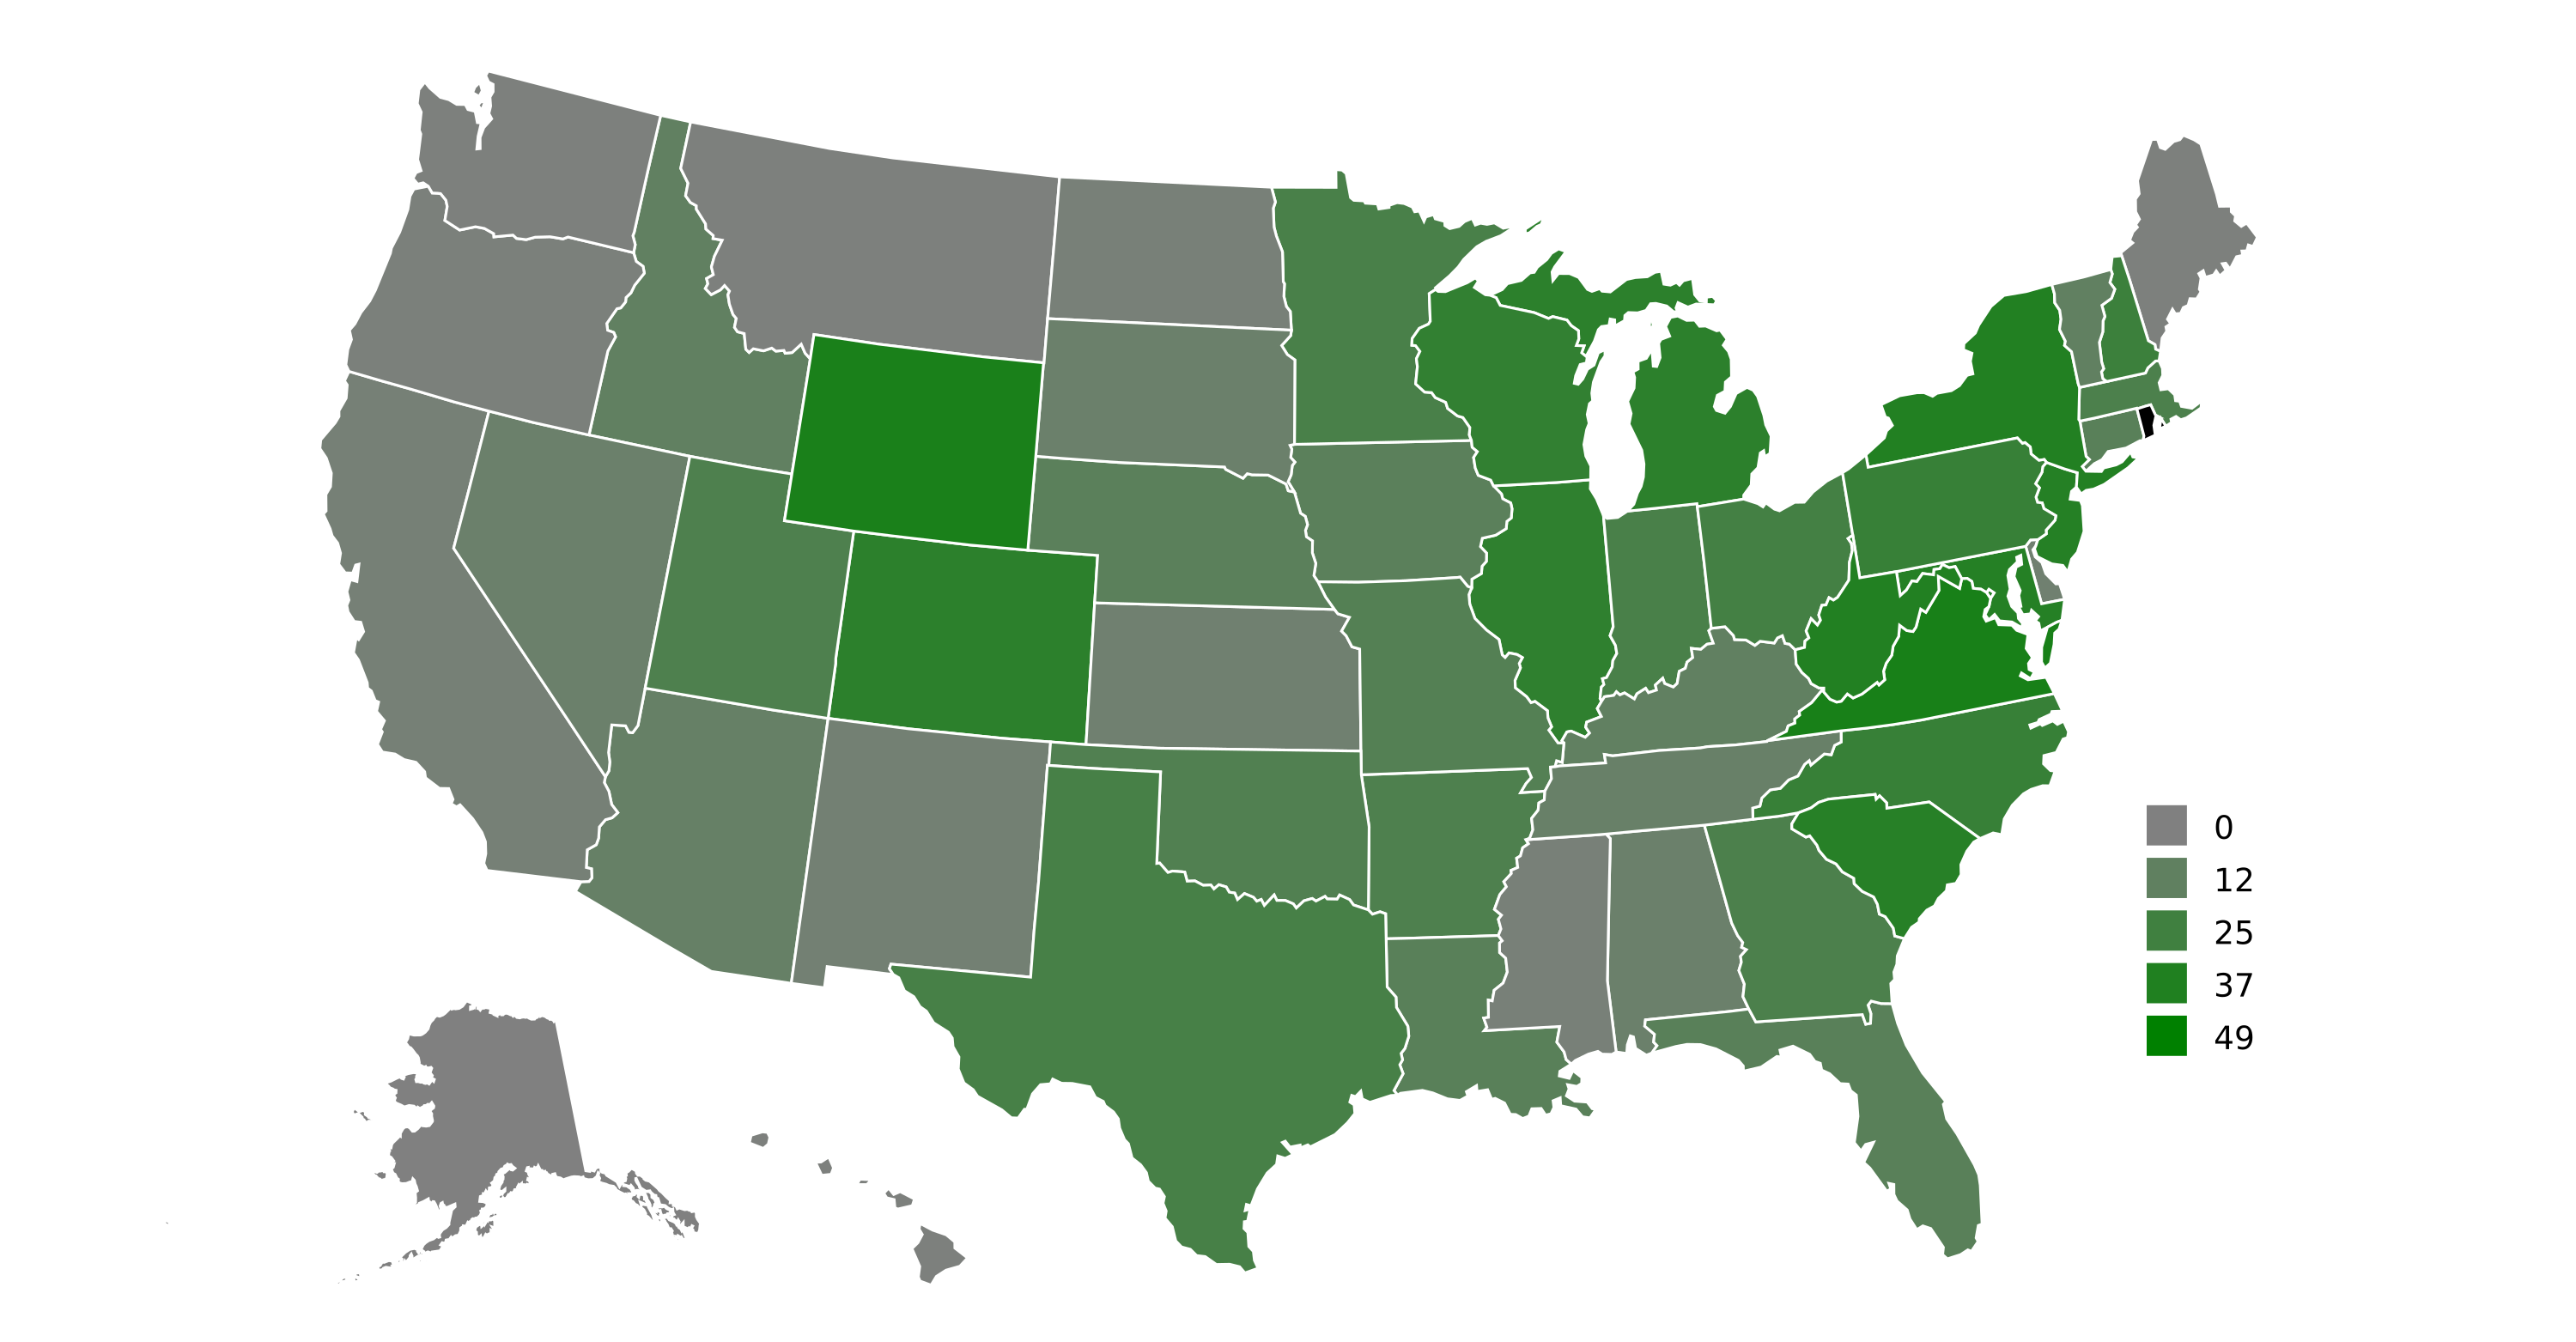
\includegraphics[width=.6\textwidth]{images/dns/analysis_auth_agg/rtt/unweighted/num_better_than_map_rtt_un.png}\\
    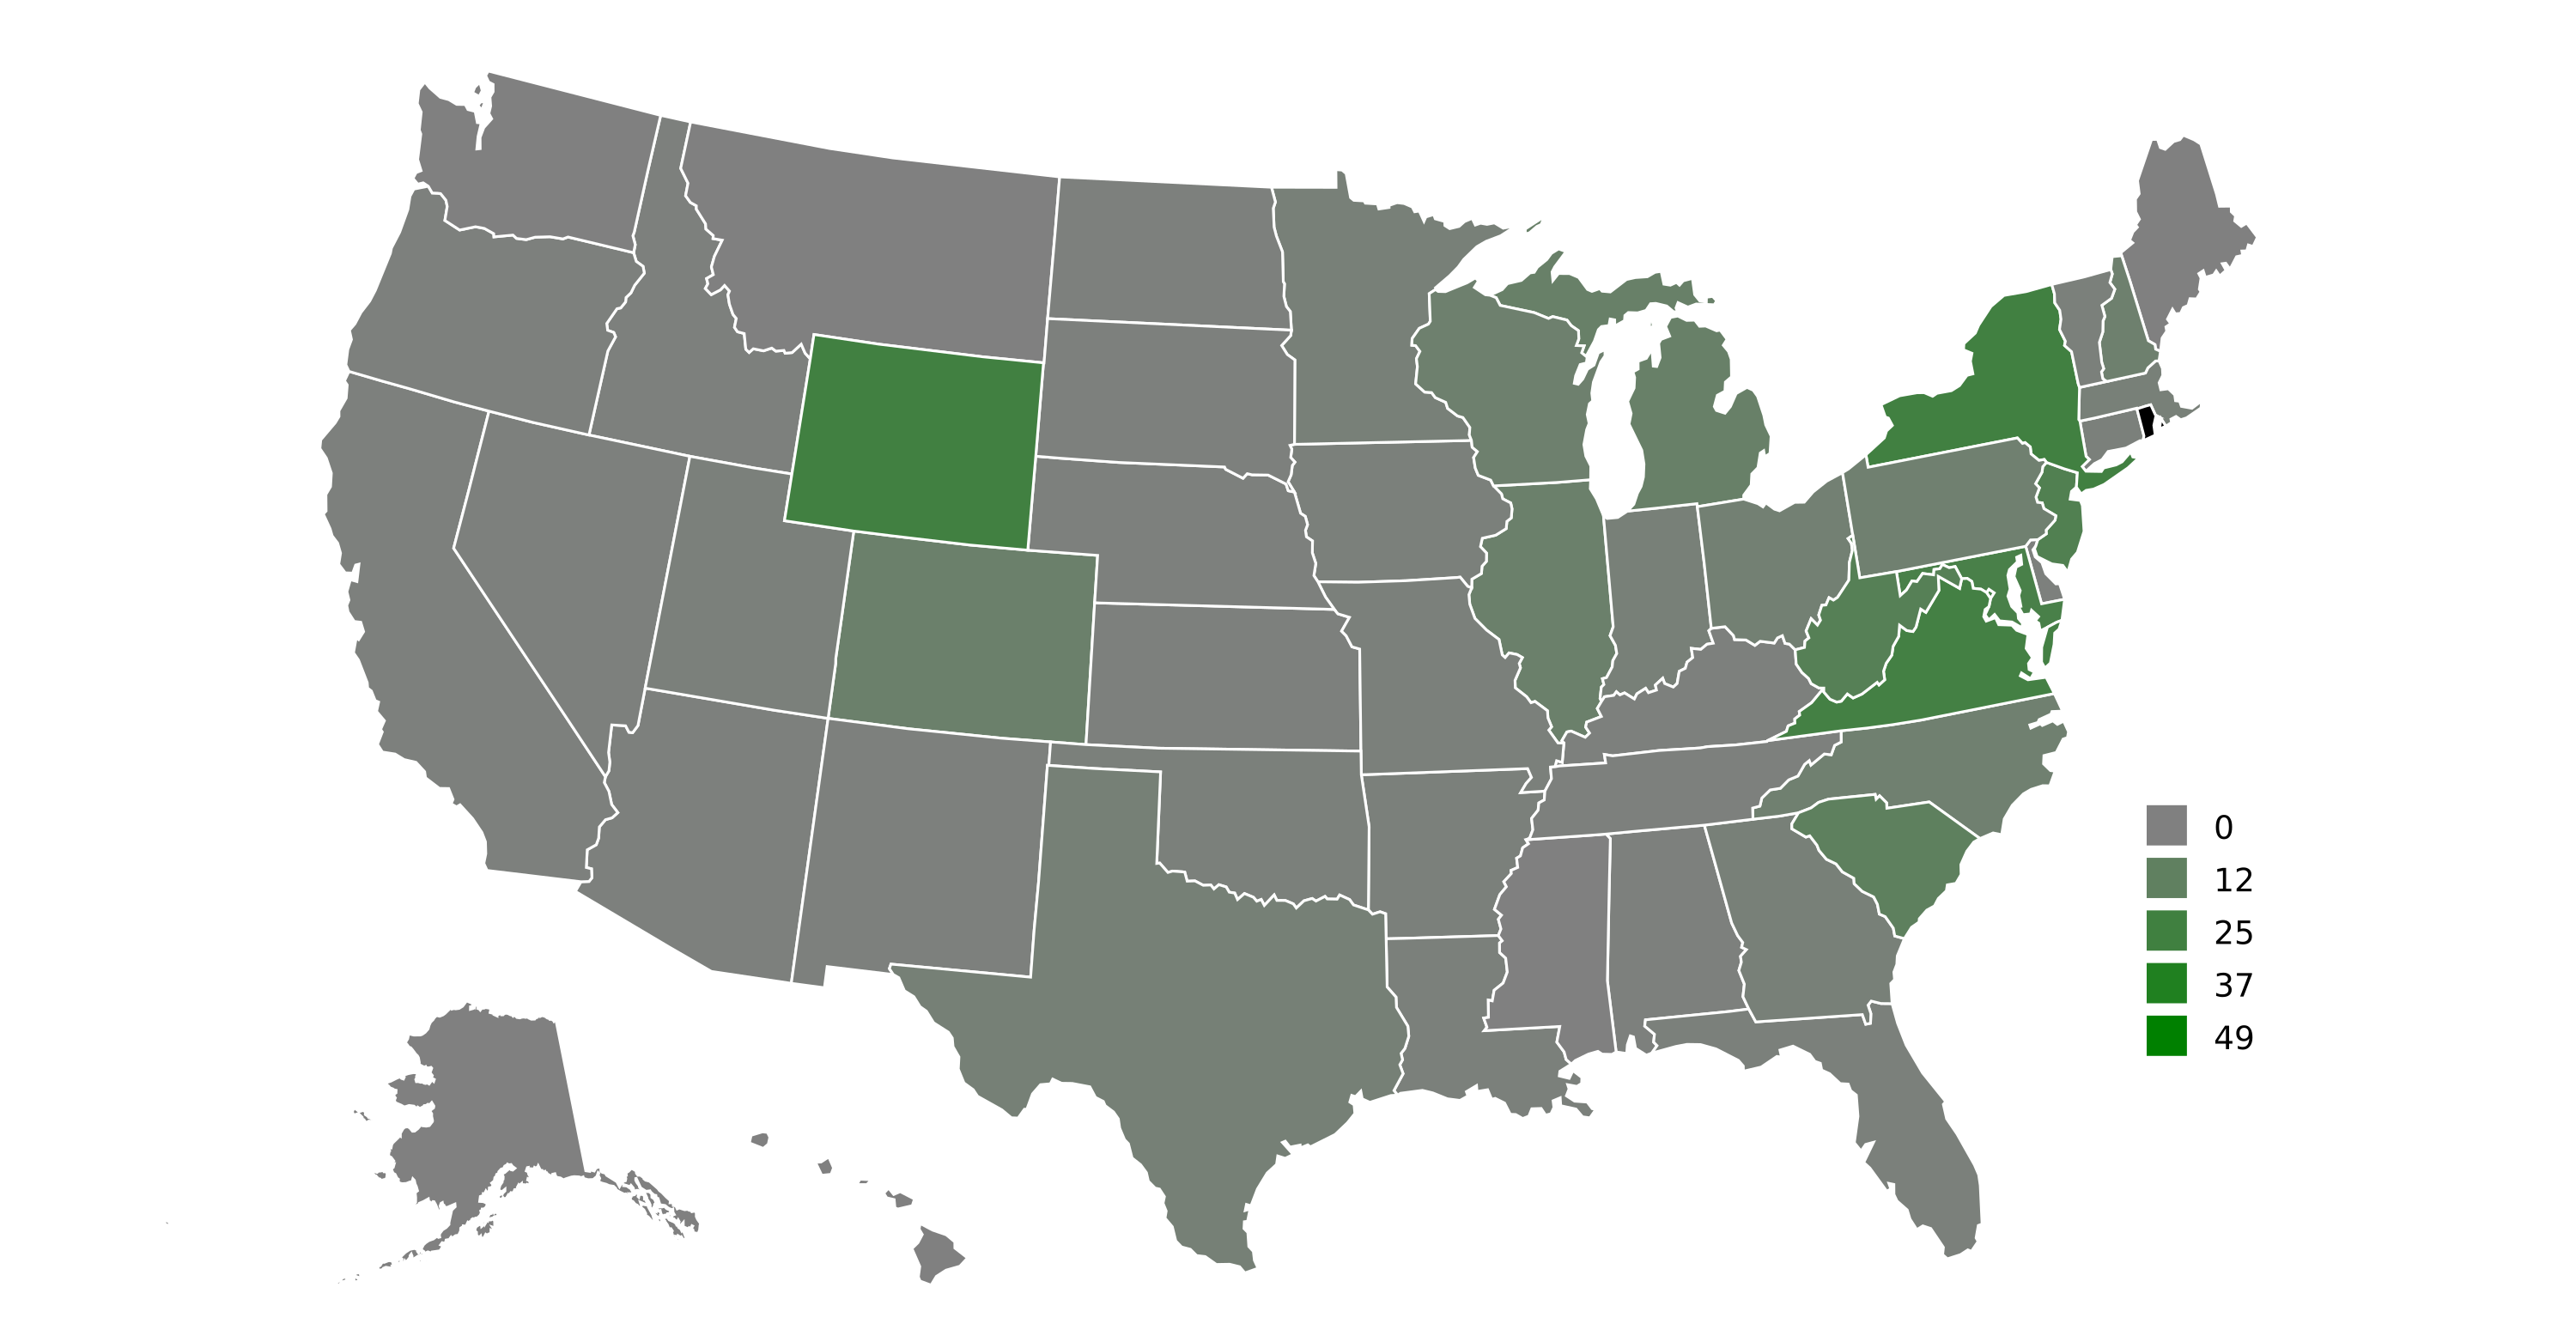
\includegraphics[width=.6\textwidth]{images/dns/analysis_auth_agg/rtt/population/num_better_than_map_rtt_pop.png}
    \caption{DNS true RTT unweighted and population weighted ``better than'' map}
    \label{fig:dns_auth_agg_num_better_map_rtt}
\end{figure}

On the other hand, the normalized maps, \cref{fig:dns_auth_agg_num_better_map_norm_rtt} show Western states performing far better than the rest of the country, although some on the East Coast do fairly well. However, much of that performance is lost when weighted by population, where Western states are far more muted. One possible explanation for this is that while the normalized metric removes the distance barrier for the West, these states are also a great distance from the denser East Coast.

\begin{figure}[htb]
    \centering
    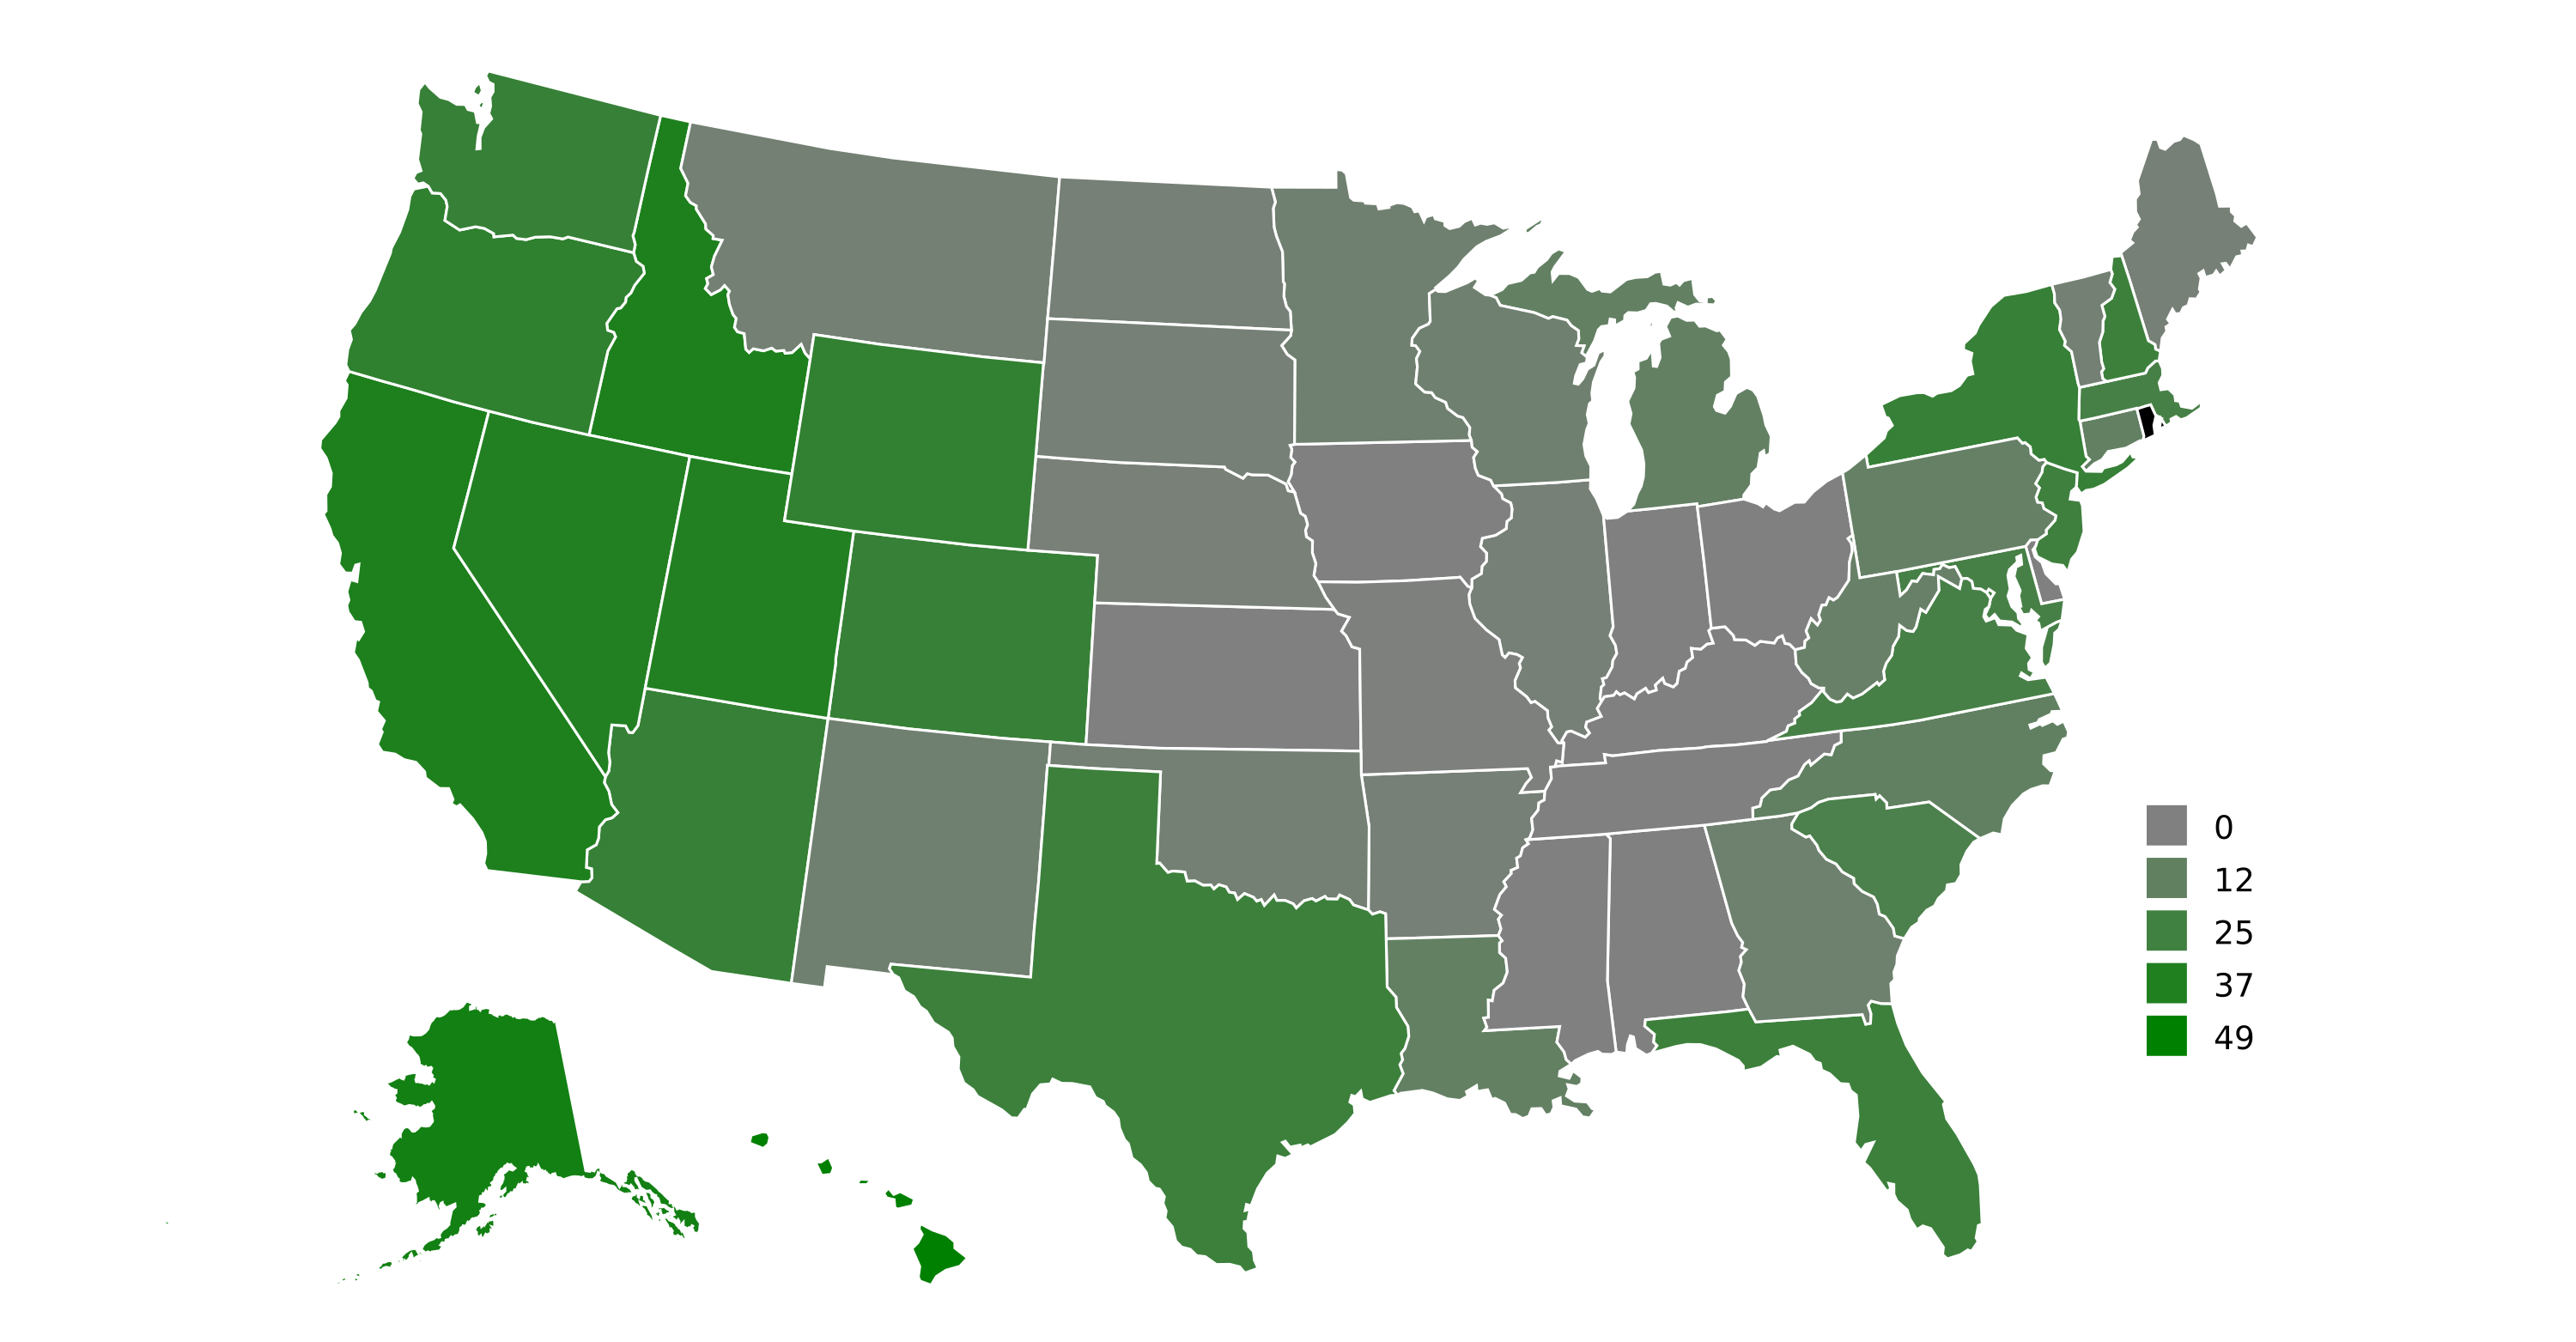
\includegraphics[width=0.6\textwidth]{images/dns/analysis_auth_agg/rtt_normalized/unweighted/num_better_than_map_norm_rtt_un.png}\\
    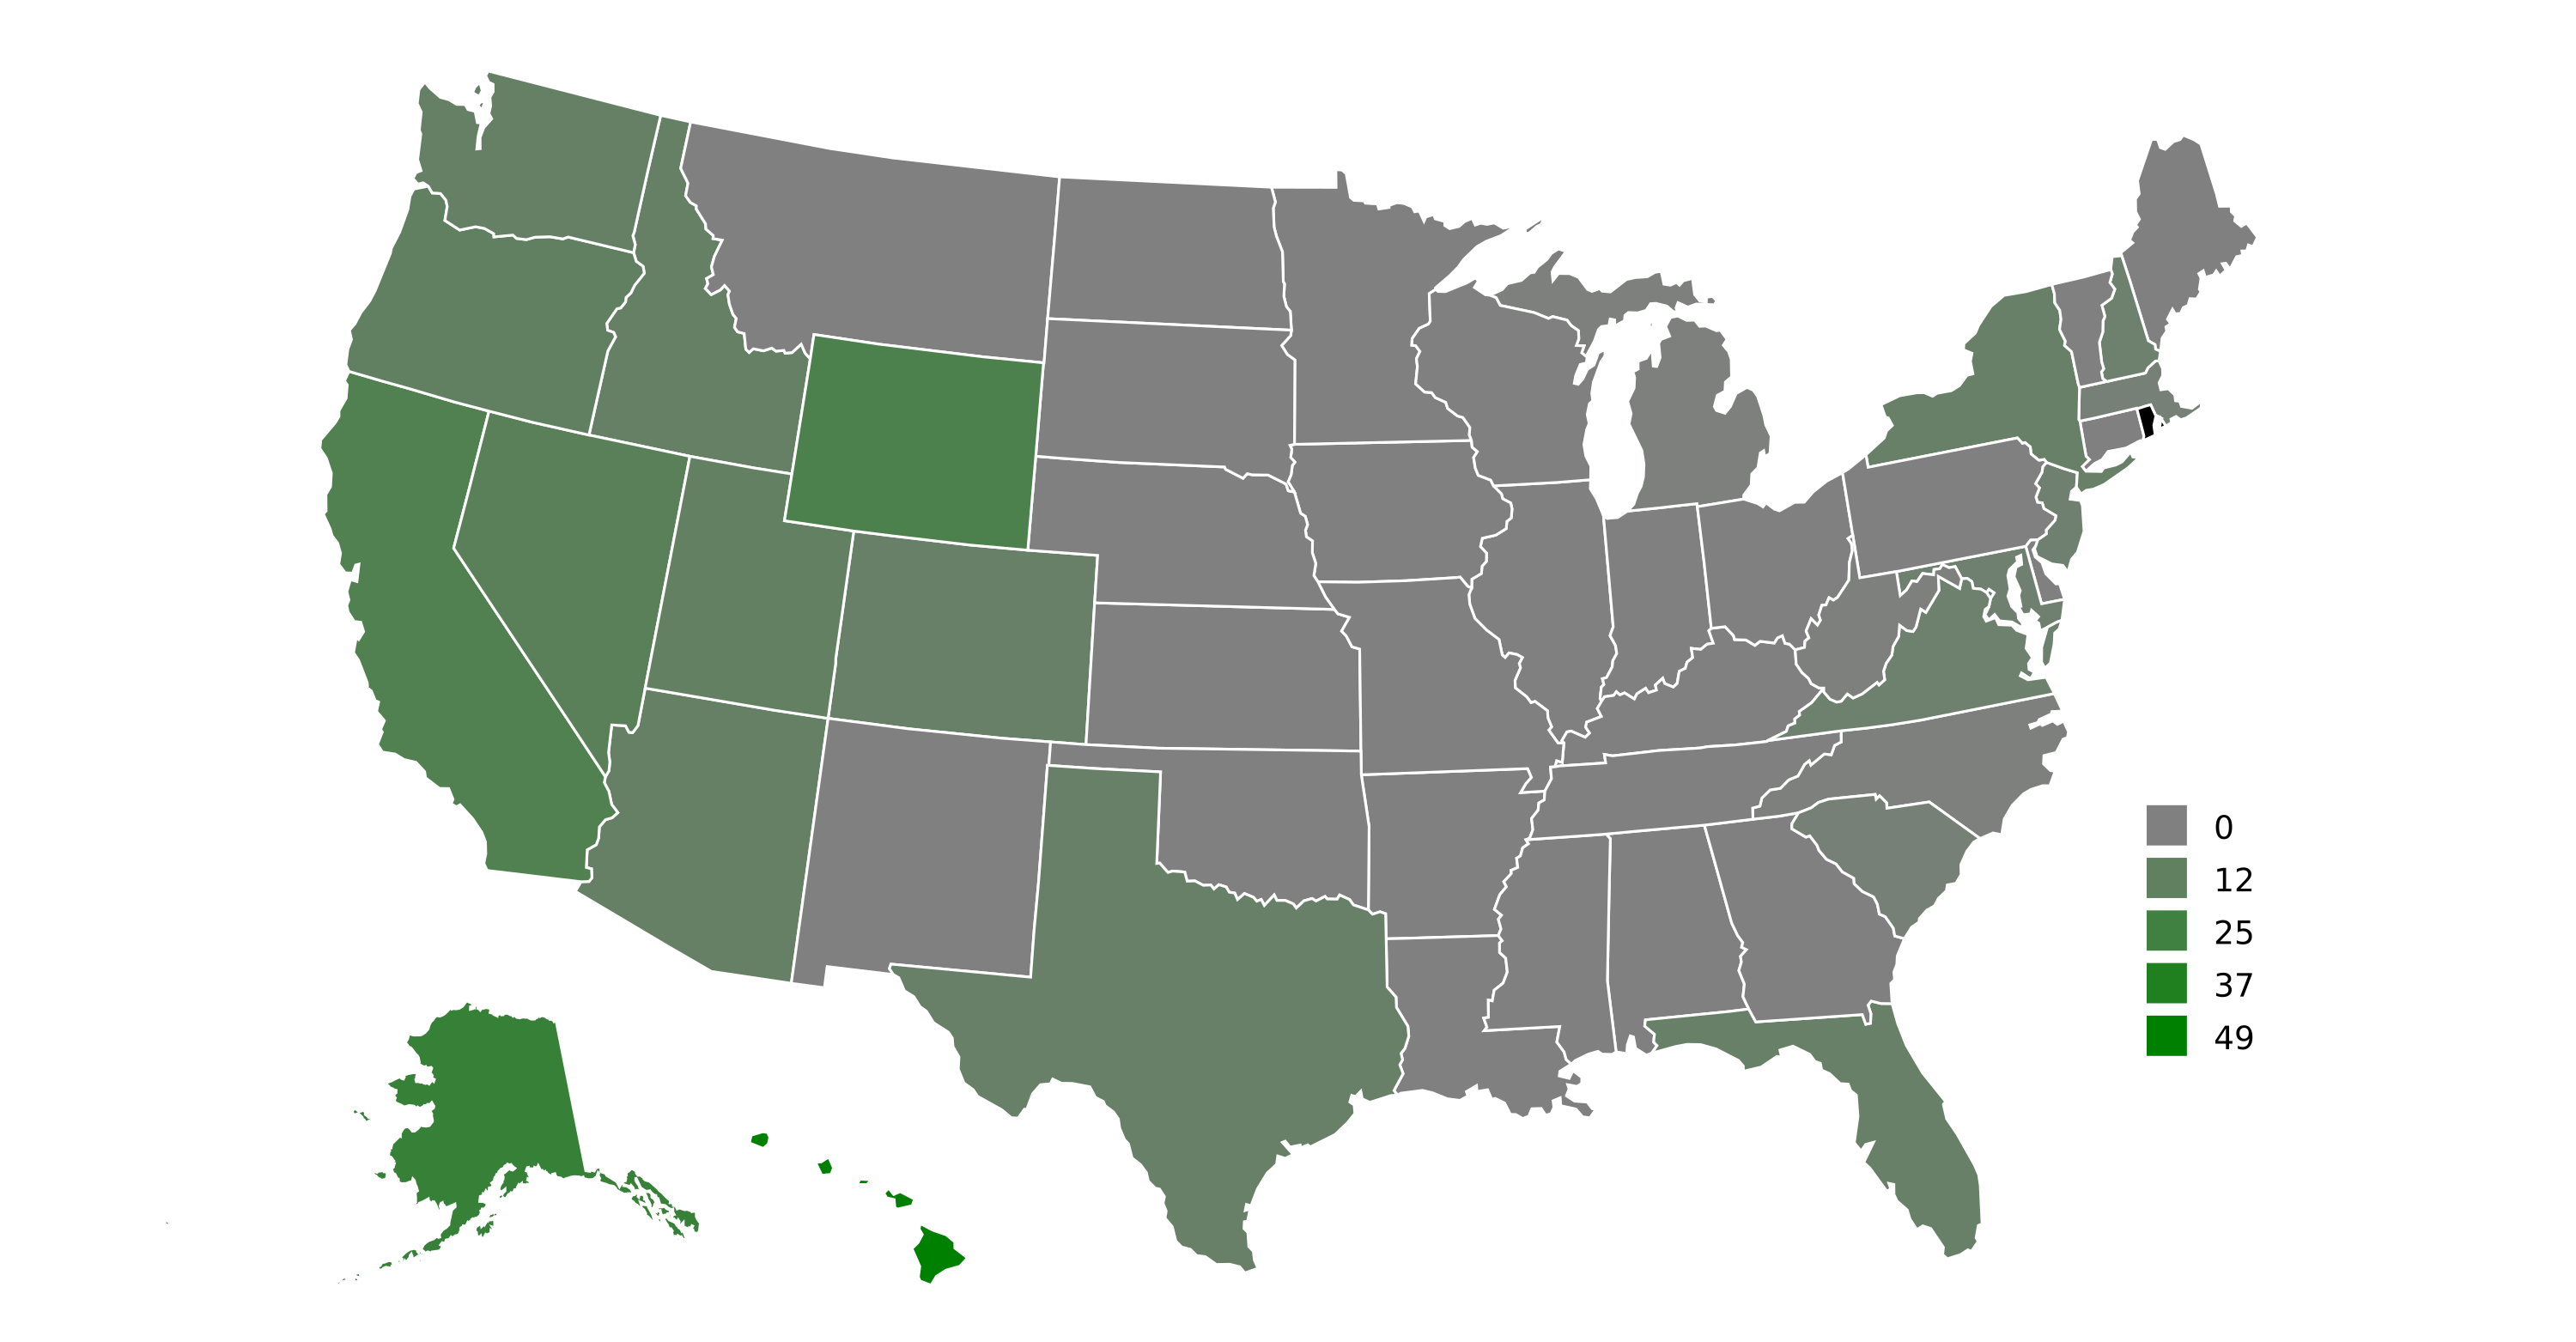
\includegraphics[width=0.6\textwidth]{images/dns/analysis_auth_agg/rtt_normalized/population/num_better_than_map_norm_rtt_pop.png}
    \caption{DNS normalized RTT unweighted  and population weighted ``better than'' map}
    \label{fig:dns_auth_agg_num_better_map_norm_rtt}
\end{figure}

Overall, these maps show that there are few meaningful conclusions that we can draw from weighting states by population: when doing so, states are far too indistinguishable from each other. However, the unweighted maps show that even if we cannot draw conclusions about specific states when eliminating the implicit \dns weighting, we can show that, for true \rtt, the East Coast and the Midwest tend to perform better as a region, as does the West Coast for normalized \rtt.

\FloatBarrier
